\documentclass{beamer}

% xcolor and define colors -------------------------
\usepackage[table]{xcolor}

% https://www.viget.com/articles/color-contrast/
\definecolor{purple}{HTML}{5601A4}
\definecolor{navy}{HTML}{0D3D56}
\definecolor{ruby}{HTML}{9a2515}
\definecolor{alice}{HTML}{107895}
\definecolor{daisy}{HTML}{EBC944}
\definecolor{coral}{HTML}{F26D21}
\definecolor{kelly}{HTML}{829356}
\definecolor{cranberry}{HTML}{E64173}
\definecolor{jet}{HTML}{131516}
\definecolor{asher}{HTML}{555F61}
\definecolor{slate}{HTML}{314F4F}

% Mixtape Sessions
\definecolor{picton-blue}{HTML}{00b7ff}
\definecolor{violet-red}{HTML}{ff3881}
\definecolor{sun}{HTML}{ffaf18}
\definecolor{electric-violet}{HTML}{871EFF}

% Main theme colors
\definecolor{accent}{HTML}{00b7ff}
\definecolor{accent2}{HTML}{871EFF}
\definecolor{gray100}{HTML}{f3f4f6}
\definecolor{gray800}{HTML}{1F292D}


% Beamer Options -------------------------------------

% Background
\setbeamercolor{background canvas}{bg = white}

% Change text margins
\setbeamersize{text margin left = 15pt, text margin right = 15pt}

% \alert
\setbeamercolor{alerted text}{fg = accent2}

% Frame title
\setbeamercolor{frametitle}{bg = white, fg = jet}
\setbeamercolor{framesubtitle}{bg = white, fg = accent}
\setbeamerfont{framesubtitle}{size = \small, shape = \itshape}

% Block
\setbeamercolor{block title}{fg = white, bg = accent2}
\setbeamercolor{block body}{fg = gray800, bg = gray100}

% Title page
\setbeamercolor{title}{fg = gray800}
\setbeamercolor{subtitle}{fg = accent}

%% Custom \maketitle and \titlepage
\setbeamertemplate{title page}
{
    %\begin{centering}
        \vspace{20mm}
        {\Large \usebeamerfont{title}\usebeamercolor[fg]{title}\inserttitle}\\
        {\large \itshape \usebeamerfont{subtitle}\usebeamercolor[fg]{subtitle}\insertsubtitle}\\ \vspace{10mm}
        {\insertauthor}\\
        {\color{asher}\small{\insertdate}}\\
    %\end{centering}
}

% Table of Contents
\setbeamercolor{section in toc}{fg = accent!70!jet}
\setbeamercolor{subsection in toc}{fg = jet}

% Button
\setbeamercolor{button}{bg = accent}

% Remove navigation symbols
\setbeamertemplate{navigation symbols}{}

% Table and Figure captions
\setbeamercolor{caption}{fg=jet!70!white}
\setbeamercolor{caption name}{fg=jet}
\setbeamerfont{caption name}{shape = \itshape}

% Bullet points

%% Fix left-margins
\settowidth{\leftmargini}{\usebeamertemplate{itemize item}}
\addtolength{\leftmargini}{\labelsep}

%% enumerate item color
\setbeamercolor{enumerate item}{fg = accent}
\setbeamerfont{enumerate item}{size = \small}
\setbeamertemplate{enumerate item}{\insertenumlabel.}

%% itemize
\setbeamercolor{itemize item}{fg = accent!70!white}
\setbeamerfont{itemize item}{size = \small}
\setbeamertemplate{itemize item}[circle]

%% right arrow for subitems
\setbeamercolor{itemize subitem}{fg = accent!60!white}
\setbeamerfont{itemize subitem}{size = \small}
\setbeamertemplate{itemize subitem}{$\rightarrow$}

\setbeamertemplate{itemize subsubitem}[square]
\setbeamercolor{itemize subsubitem}{fg = jet}
\setbeamerfont{itemize subsubitem}{size = \small}


% Special characters

\usepackage{collectbox}

\makeatletter
\newcommand{\mybox}{%
    \collectbox{%
        \setlength{\fboxsep}{1pt}%
        \fbox{\BOXCONTENT}%
    }%
}
\makeatother





% Links ----------------------------------------------

\usepackage{hyperref}
\hypersetup{
  colorlinks = true,
  linkcolor = accent2,
  filecolor = accent2,
  urlcolor = accent2,
  citecolor = accent2,
}


% Line spacing --------------------------------------
\usepackage{setspace}
\setstretch{1.1}


% \begin{columns} -----------------------------------
\usepackage{multicol}


% Fonts ---------------------------------------------
% Beamer Option to use custom fonts
\usefonttheme{professionalfonts}

% \usepackage[utopia, smallerops, varg]{newtxmath}
% \usepackage{utopia}
\usepackage[sfdefault,light]{roboto}

% Small adjustments to text kerning
\usepackage{microtype}



% Remove annoying over-full box warnings -----------
\vfuzz2pt
\hfuzz2pt


% Table of Contents with Sections
\setbeamerfont{myTOC}{series=\bfseries, size=\Large}
\AtBeginSection[]{
        \frame{
            \frametitle{Roadmap}
            \tableofcontents[current]
        }
    }


% Tables -------------------------------------------
% Tables too big
% \begin{adjustbox}{width = 1.2\textwidth, center}
\usepackage{adjustbox}
\usepackage{array}
\usepackage{threeparttable, booktabs, adjustbox}

% Fix \input with tables
% \input fails when \\ is at end of external .tex file
\makeatletter
\let\input\@@input
\makeatother

% Tables too narrow
% \begin{tabularx}{\linewidth}{cols}
% col-types: X - center, L - left, R -right
% Relative scale: >{\hsize=.8\hsize}X/L/R
\usepackage{tabularx}
\newcolumntype{L}{>{\raggedright\arraybackslash}X}
\newcolumntype{R}{>{\raggedleft\arraybackslash}X}
\newcolumntype{C}{>{\centering\arraybackslash}X}

% Figures

% \imageframe{img_name} -----------------------------
% from https://github.com/mattjetwell/cousteau
\newcommand{\imageframe}[1]{%
    \begin{frame}[plain]
        \begin{tikzpicture}[remember picture, overlay]
            \node[at = (current page.center), xshift = 0cm] (cover) {%
                \includegraphics[keepaspectratio, width=\paperwidth, height=\paperheight]{#1}
            };
        \end{tikzpicture}
    \end{frame}%
}

% subfigures
\usepackage{subfigure}


% Highlight slide -----------------------------------
% \begin{transitionframe} Text \end{transitionframe}
% from paulgp's beamer tips
\newenvironment{transitionframe}{
    \setbeamercolor{background canvas}{bg=accent!40!black}
    \begin{frame}\color{accent!10!white}\LARGE\centering
}{
    \end{frame}
}


% Table Highlighting --------------------------------
% Create top-left and bottom-right markets in tabular cells with a unique matching id and these commands will outline those cells
\usepackage[beamer,customcolors]{hf-tikz}
\usetikzlibrary{calc}
\usetikzlibrary{fit,shapes.misc}

% To set the hypothesis highlighting boxes red.
\newcommand\marktopleft[1]{%
    \tikz[overlay,remember picture]
        \node (marker-#1-a) at (0,1.5ex) {};%
}
\newcommand\markbottomright[1]{%
    \tikz[overlay,remember picture]
        \node (marker-#1-b) at (0,0) {};%
    \tikz[accent!80!jet, ultra thick, overlay, remember picture, inner sep=4pt]
        \node[draw, rectangle, fit=(marker-#1-a.center) (marker-#1-b.center)] {};%
}

\usepackage{breqn} % Breaks lines

\usepackage{tikz}
\usetikzlibrary{positioning}

\usepackage{amsmath}
\usepackage{mathtools}

\usepackage{pdfpages} % \includepdf

\usepackage{listings} % R code
\usepackage{verbatim} % verbatim

% Video stuff
\usepackage{media9}

% packages for bibs and cites
\usepackage{natbib}
\usepackage{har2nat}
\newcommand{\possessivecite}[1]{\citeauthor{#1}'s \citeyearpar{#1}}
\usepackage{breakcites}
\usepackage{alltt}

% Setup math operators
\DeclareMathOperator{\E}{E} \DeclareMathOperator{\tr}{tr} \DeclareMathOperator{\se}{se} \DeclareMathOperator{\I}{I} \DeclareMathOperator{\sign}{sign} \DeclareMathOperator{\supp}{supp} \DeclareMathOperator{\plim}{plim}
\DeclareMathOperator*{\dlim}{\mathnormal{d}\mkern2mu-lim}
\newcommand\independent{\protect\mathpalette{\protect\independenT}{\perp}}
   \def\independenT#1#2{\mathrel{\rlap{$#1#2$}\mkern2mu{#1#2}}}
\newcommand*\colvec[1]{\begin{pmatrix}#1\end{pmatrix}}

\newcommand{\myurlshort}[2]{\href{#1}{\textcolor{gray}{\textsf{#2}}}}


\begin{document}

\imageframe{./lecture_includes/slide_banner.pdf}


% ---- Content ----

\section{Two Contemporary Examples}

\subsection{Facebook and Mental Health}

\begin{frame}{Bringing them together}

\begin{itemize}

\item Now we will look at a couple of studies using differential timing to understand both the studies (as a nice break), but also how they approached what we covered
	\begin{enumerate}
	\item Braghieri, Levy and Makarin (2022), ``Social Media and Mental Health'', \emph{American Economic Review}, 112(11): 3660-3693
	\item Brynjolfsson, Li and Raymond (2023), ``Generative AI at Work'', \emph{NBER Working Paper 31161}
	\end{enumerate}
\item I also love these papers because what I hope to do is suggest why TWFE seems problematic in the first, but weirdly, not the second

\end{itemize}

\end{frame}


\begin{frame}
\begin{center}
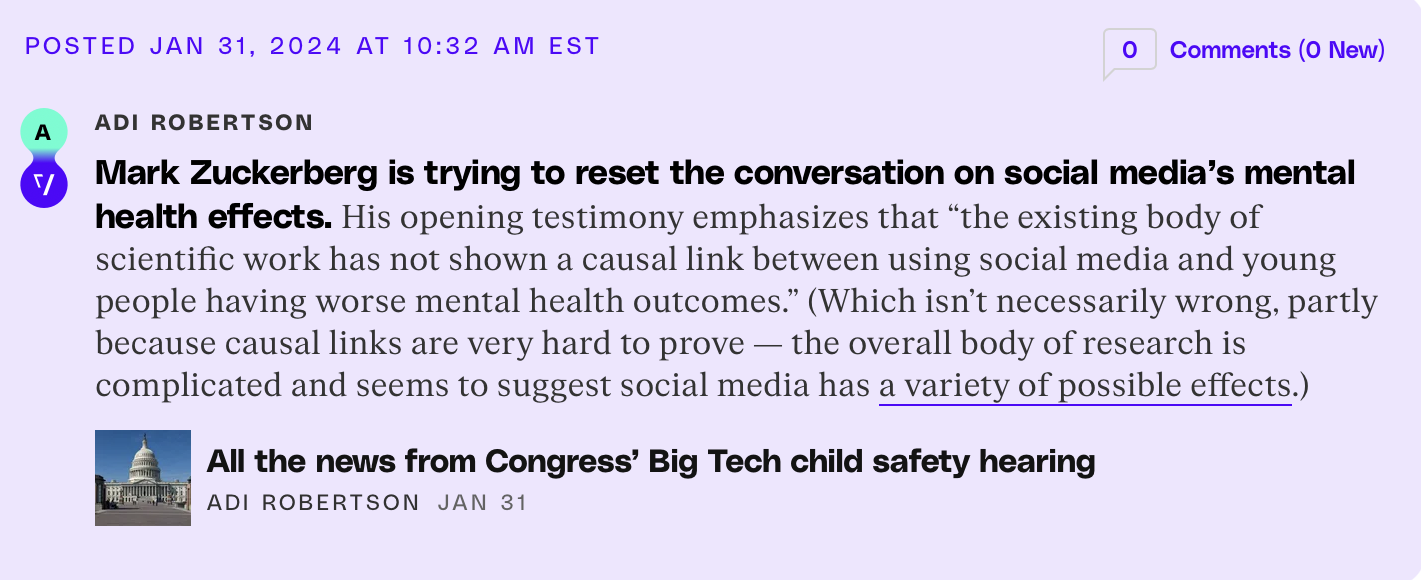
\includegraphics[scale=0.35]{./lecture_includes/facebook_quote}
\end{center}
\end{frame}



\begin{frame}{Mental health and Social Media}

\begin{itemize}
\item Unclear what he means; he may mean there is no experimental evidence
\item Very difficult to imagine a randomized experiment being realistic or ethical 
\item Once the claim out there is that it is harmful, Institutional Review Boards likely wouldn't approve it
\item Herein is a reason we so often focus on quasi-experimental approaches -- for many policy questions, it's the only way 


\end{itemize}

\end{frame}

\begin{frame}{Reviewing the contribution}

\begin{itemize}

\item Premiere journals are looking for important research questions, high quality data and appropriate research designs (if causal)
\item My observations are about the paper's contribution
	\begin{enumerate}
	\item Social media platforms impact on youth mental health is a major policy question and difficult to answer (see Zuckerberg testifying before Congress about it)
	\item Meticulous data collection with ingenious linkages (but which are increasingly common)
	\item Quasi-experimental research design using differential timing difference-in-differences
	\item Data visualization from event studies (appropriately specified) are compelling
	\end{enumerate}

\end{itemize}

\end{frame}


\begin{frame}{Overview}

\begin{itemize}
\item Facebook (``theFacebook'') initially targeted different American universities from 2004 to 2006 \emph{at different points in time}
\item They found an online data source that allowed them to pin point precisely when a university was ``treated'' with theFacebook
\item They then linked that data with a longrunning health survey of college students (both before and after) in a very clever way
\item Estimated the effect of a new social media platform's presence at a university on student revealed mental health problems

\end{itemize}

\end{frame}




\begin{frame}{Five elements of a strong DiD}


\begin{enumerate}

\item \textbf{Bite}: \textcolor{red}{Nothing}. They cannot really show much here.  No data on Facebook usage.  They had to rely on anecdote and Facebook as a ``first mover'', but there had been Friendster and MySpace so this does weaken the paper maybe. More intent-to-treat
\item \textbf{Main Results}: Very strong evidence, mostly expressed using rich survey data and questions transformed into z-scores (standard deviations)
\item \textbf{Falsifications}: \textcolor{red}{None}. Authors do not perform falsifications. Remember Miller, Johnson and Wherry looking at Medicaid's effect on Medicare eligible population?  There isn't anything like that here.
\item \textbf{Event studies}: Extremely compelling evidence and robustness across a half dozen different models
\item \textbf{Mechanism}: \textcolor{red}{Speculative but let's see what you think}

\end{enumerate}

\end{frame}








\begin{frame}{Main Specification: TWFE}

\begin{equation}
Y_{icgt} = \alpha_g + \delta_t + \beta \times Facebook_{gt} + X_i \times \gamma + X_c \times \psi + \varepsilon_{icgt}
\end{equation}

\bigskip

\begin{itemize}
\item Authors in 2022 \emph{American Economic Review} made a TWFE specification their main model. 
\item Why given they will also estimate the robust methods?  
\item One of them told me that when they submitted, DiD literacy was much lower than it is now, and they could not take for granted people would know this material -- so they present the new work as ``robustness''
\item Does not mean that this is true now, but it's something to remember -- know your audience, anticipate their expectations and write accordingly 
\item Dan and Mark, what's your thoughts as editors about this?
\end{itemize}

\end{frame}


\begin{frame}{Data on Facebook}

\begin{itemize}

\item When does Facebook appear at a school?  
	\begin{itemize}
	\item Facebook only publishes a fraction of that information
	\item They came up with a workaround
	\end{itemize}
\item The Wayback Machine has been taking almost daily photographs of every website since the Internet's beginning -- including the frontpage of ``TheFacebook''
\item This is a very useful website for you to know about -- we also used it in a recent publication of mine (Cunningham, DeAngelo and Tripp 2023)

\end{itemize}

\end{frame}

\begin{frame}
\begin{center}
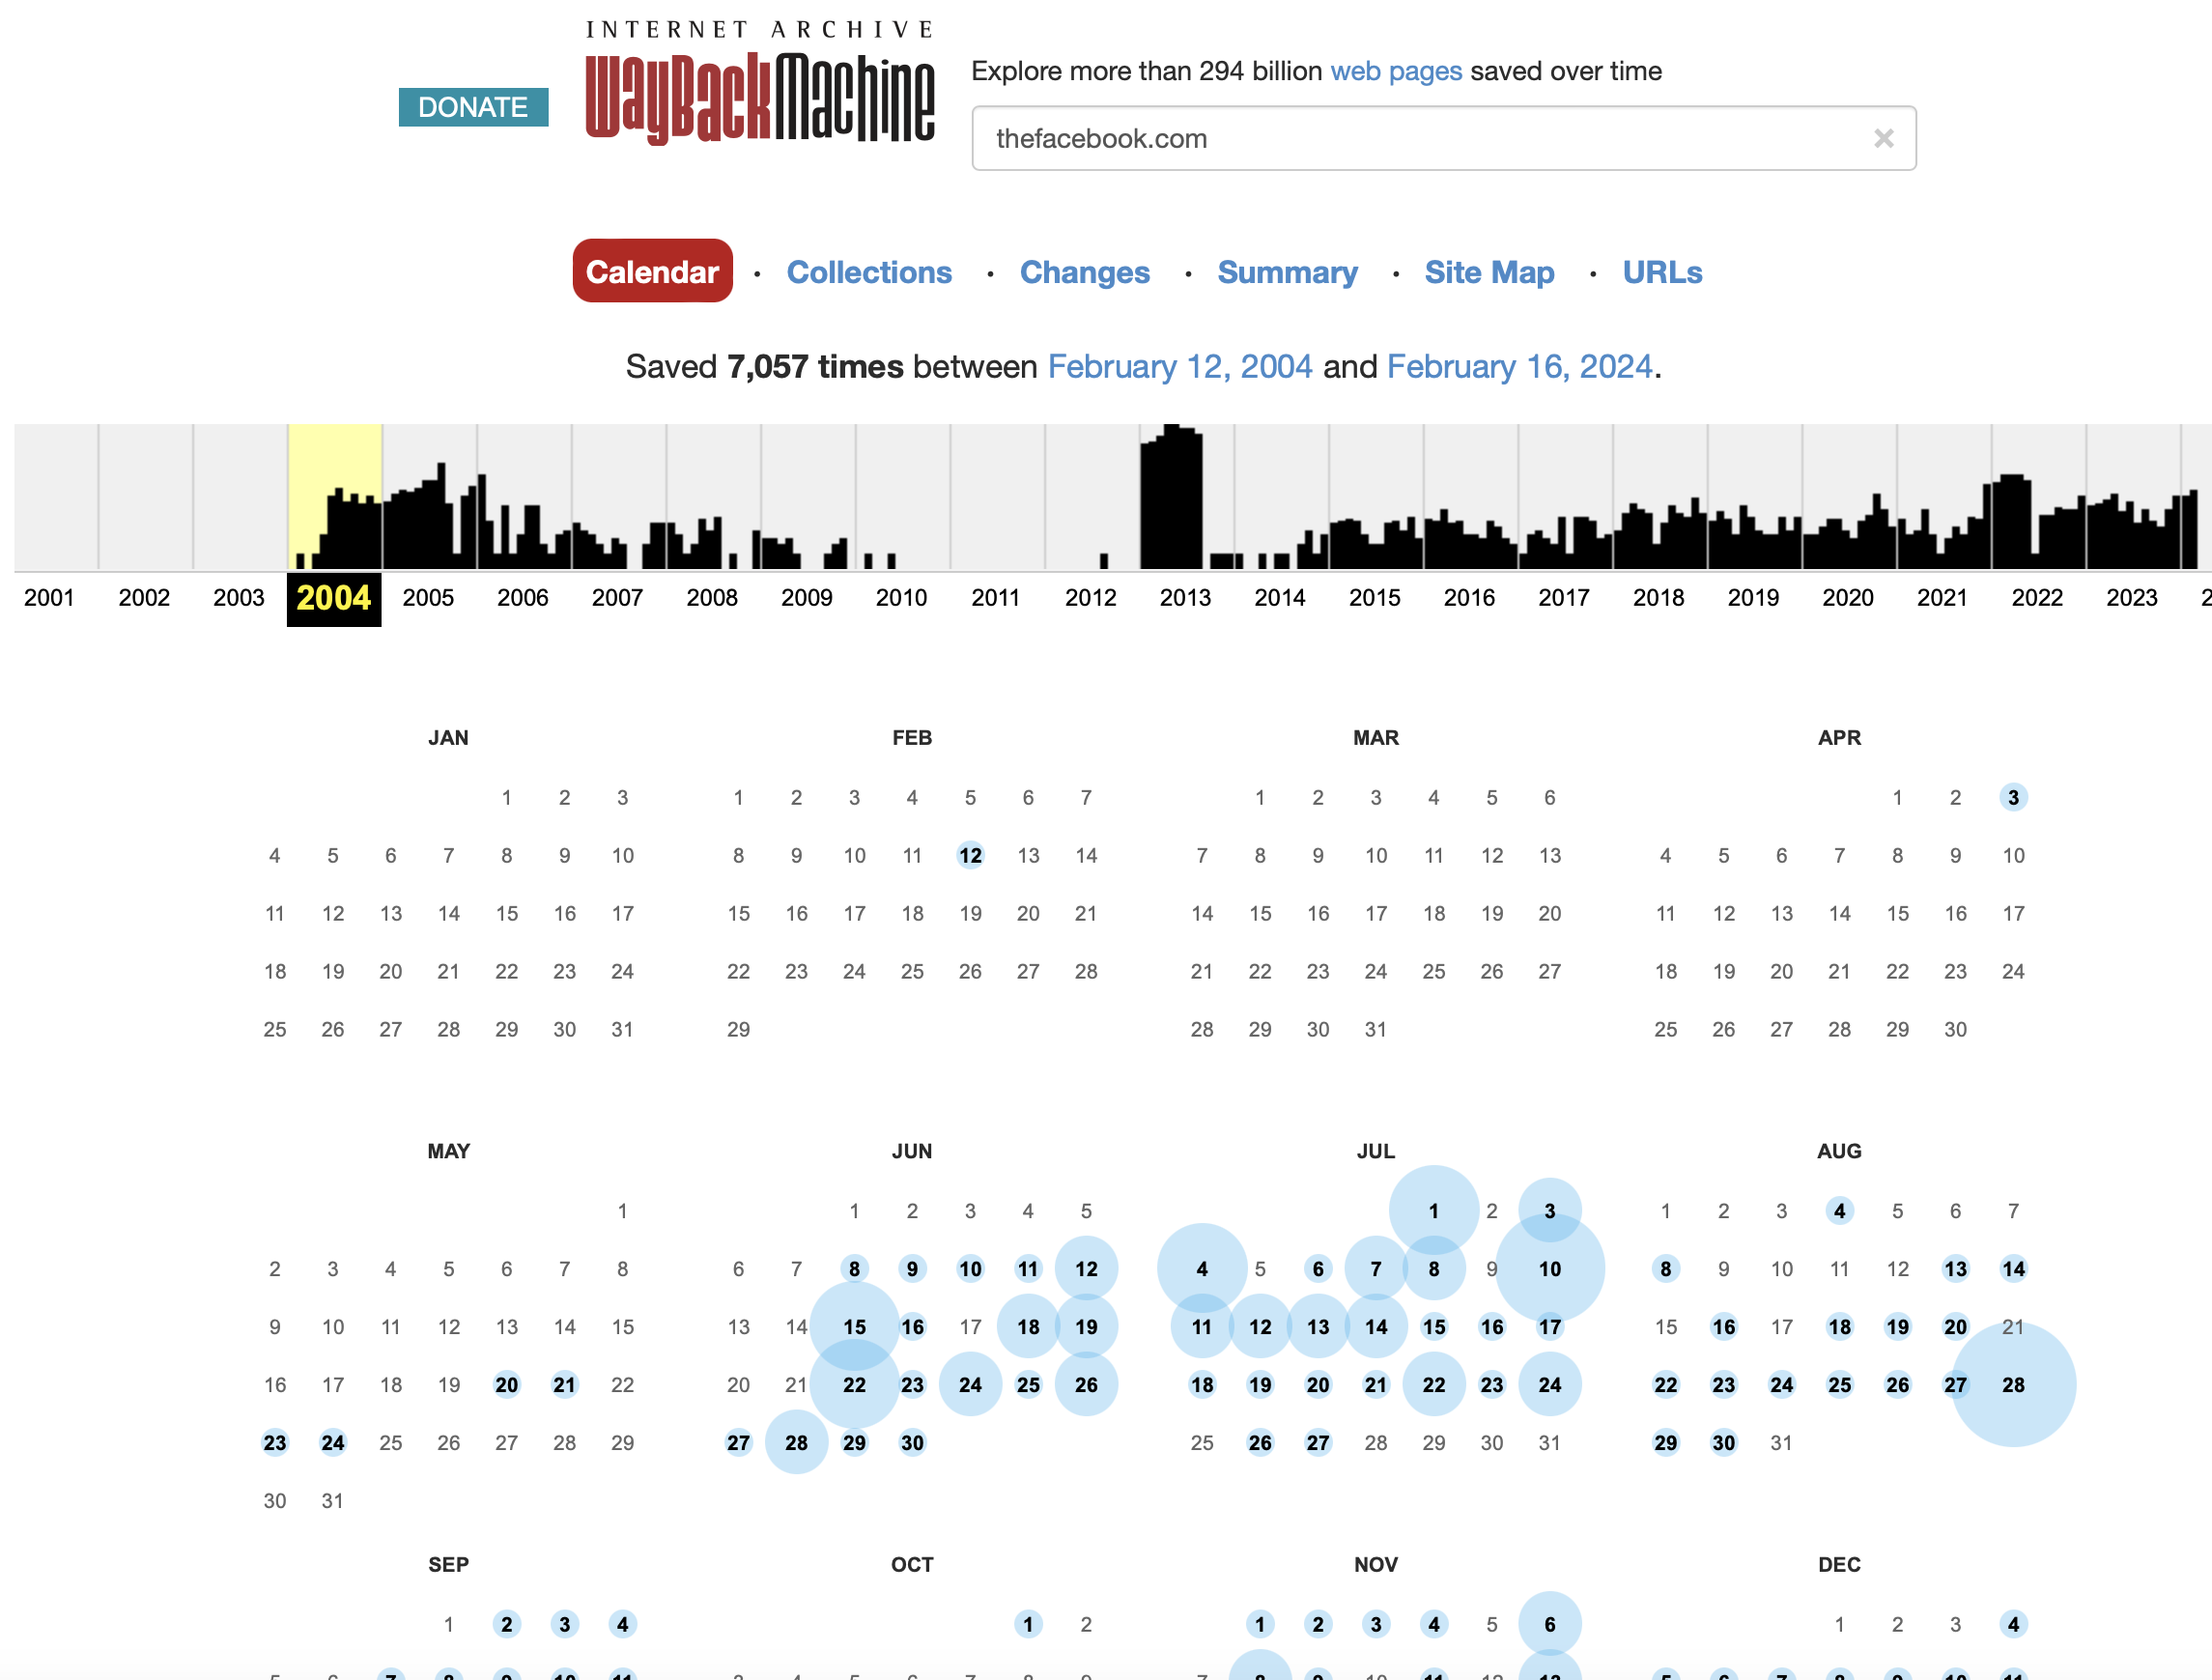
\includegraphics[scale=0.25]{./lecture_includes/wayback1}
\end{center}
\end{frame}

\begin{frame}{Differential Timing?}

\begin{itemize}

\item The Wayback Machine only lets you see a website at different points in time (more or less the universe though)
\item But how are they going to take a website to support a difference-in-differences design?
\item Look at what was on the front page 

\end{itemize}

\end{frame}

\begin{frame}
\begin{center}
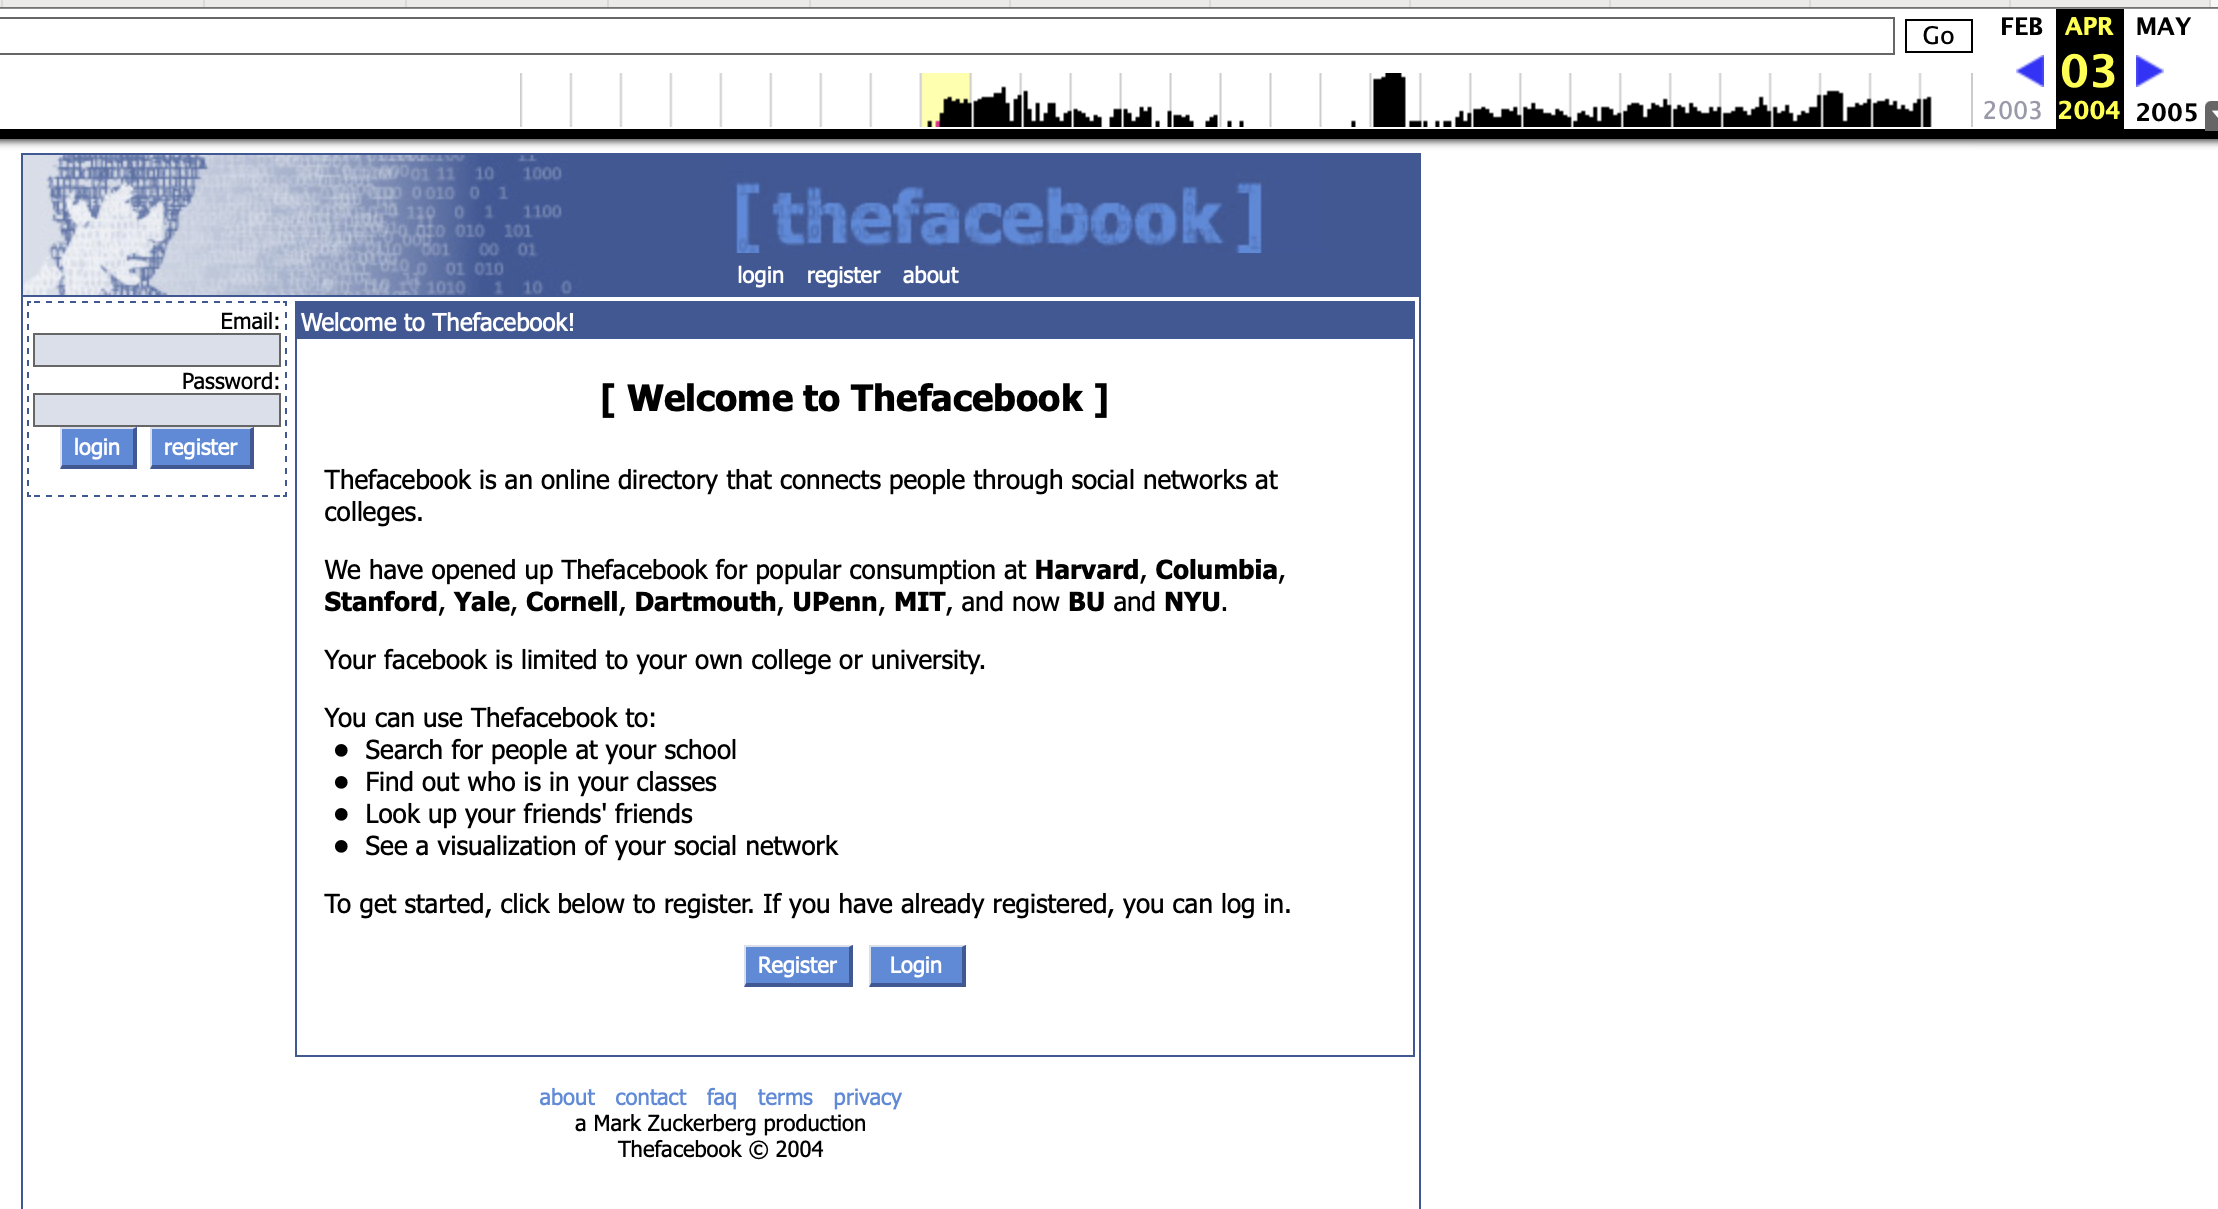
\includegraphics[scale=0.35]{./lecture_includes/wayback2}
\end{center}
\end{frame}

\begin{frame}
\begin{center}
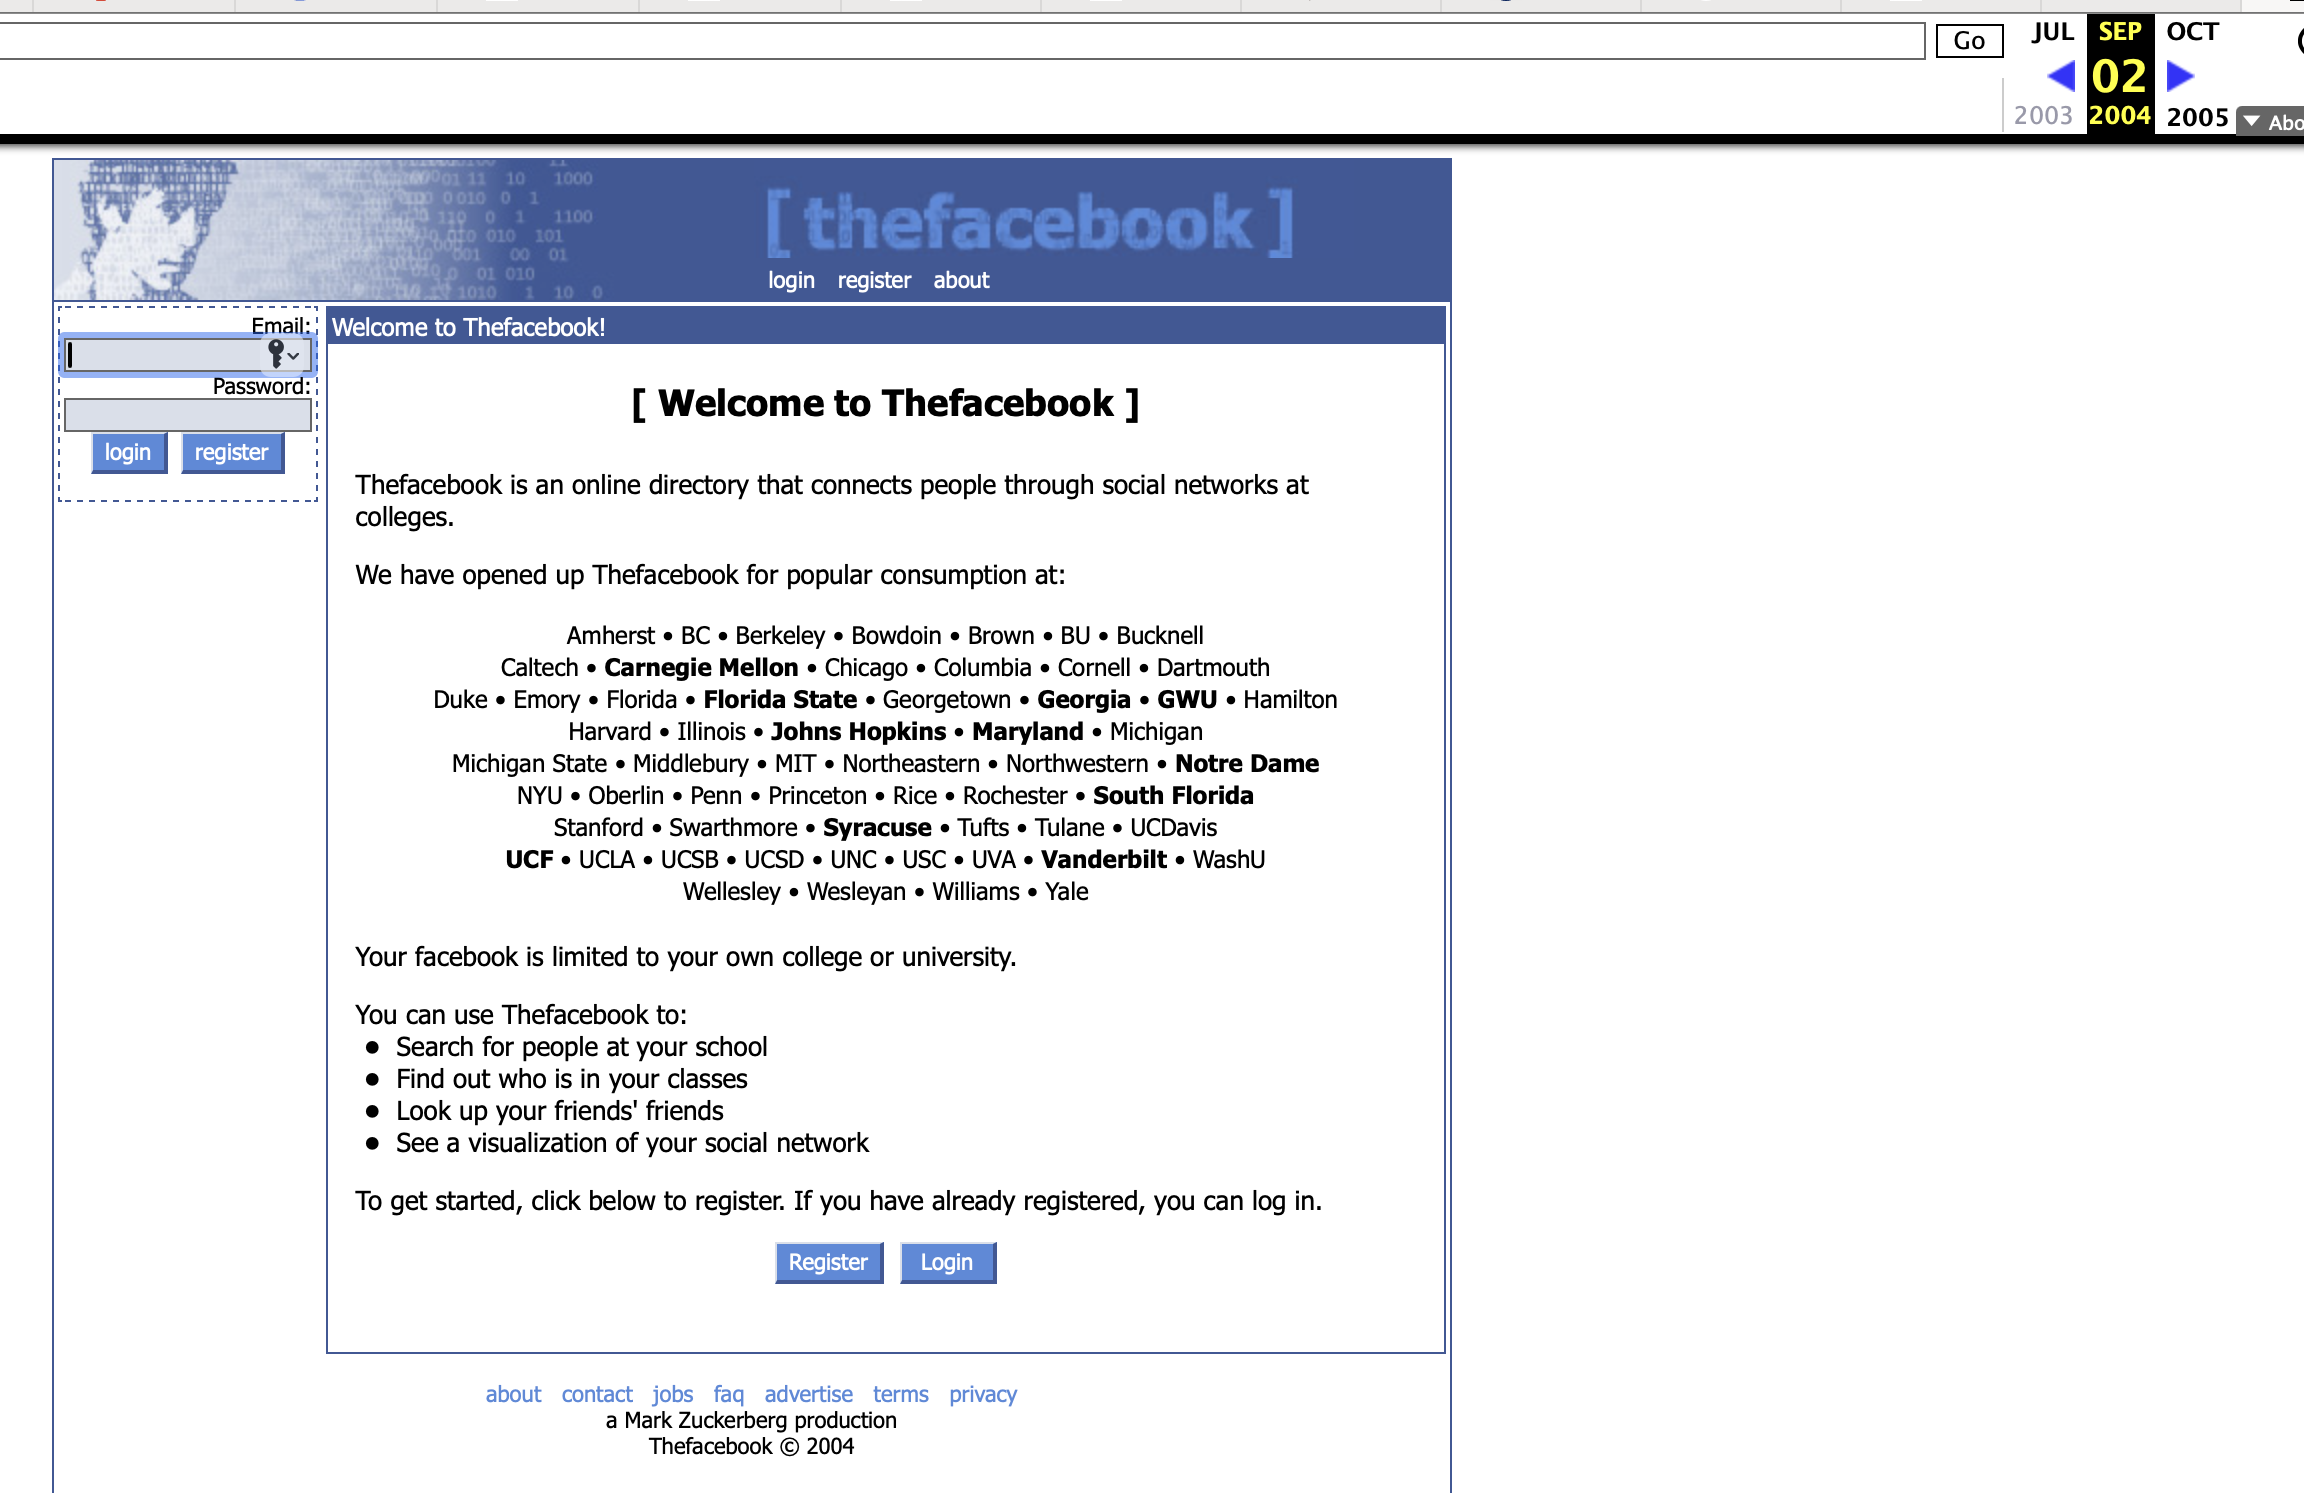
\includegraphics[scale=0.25]{./lecture_includes/wayback3}
\end{center}
\end{frame}

\begin{frame}
\begin{center}
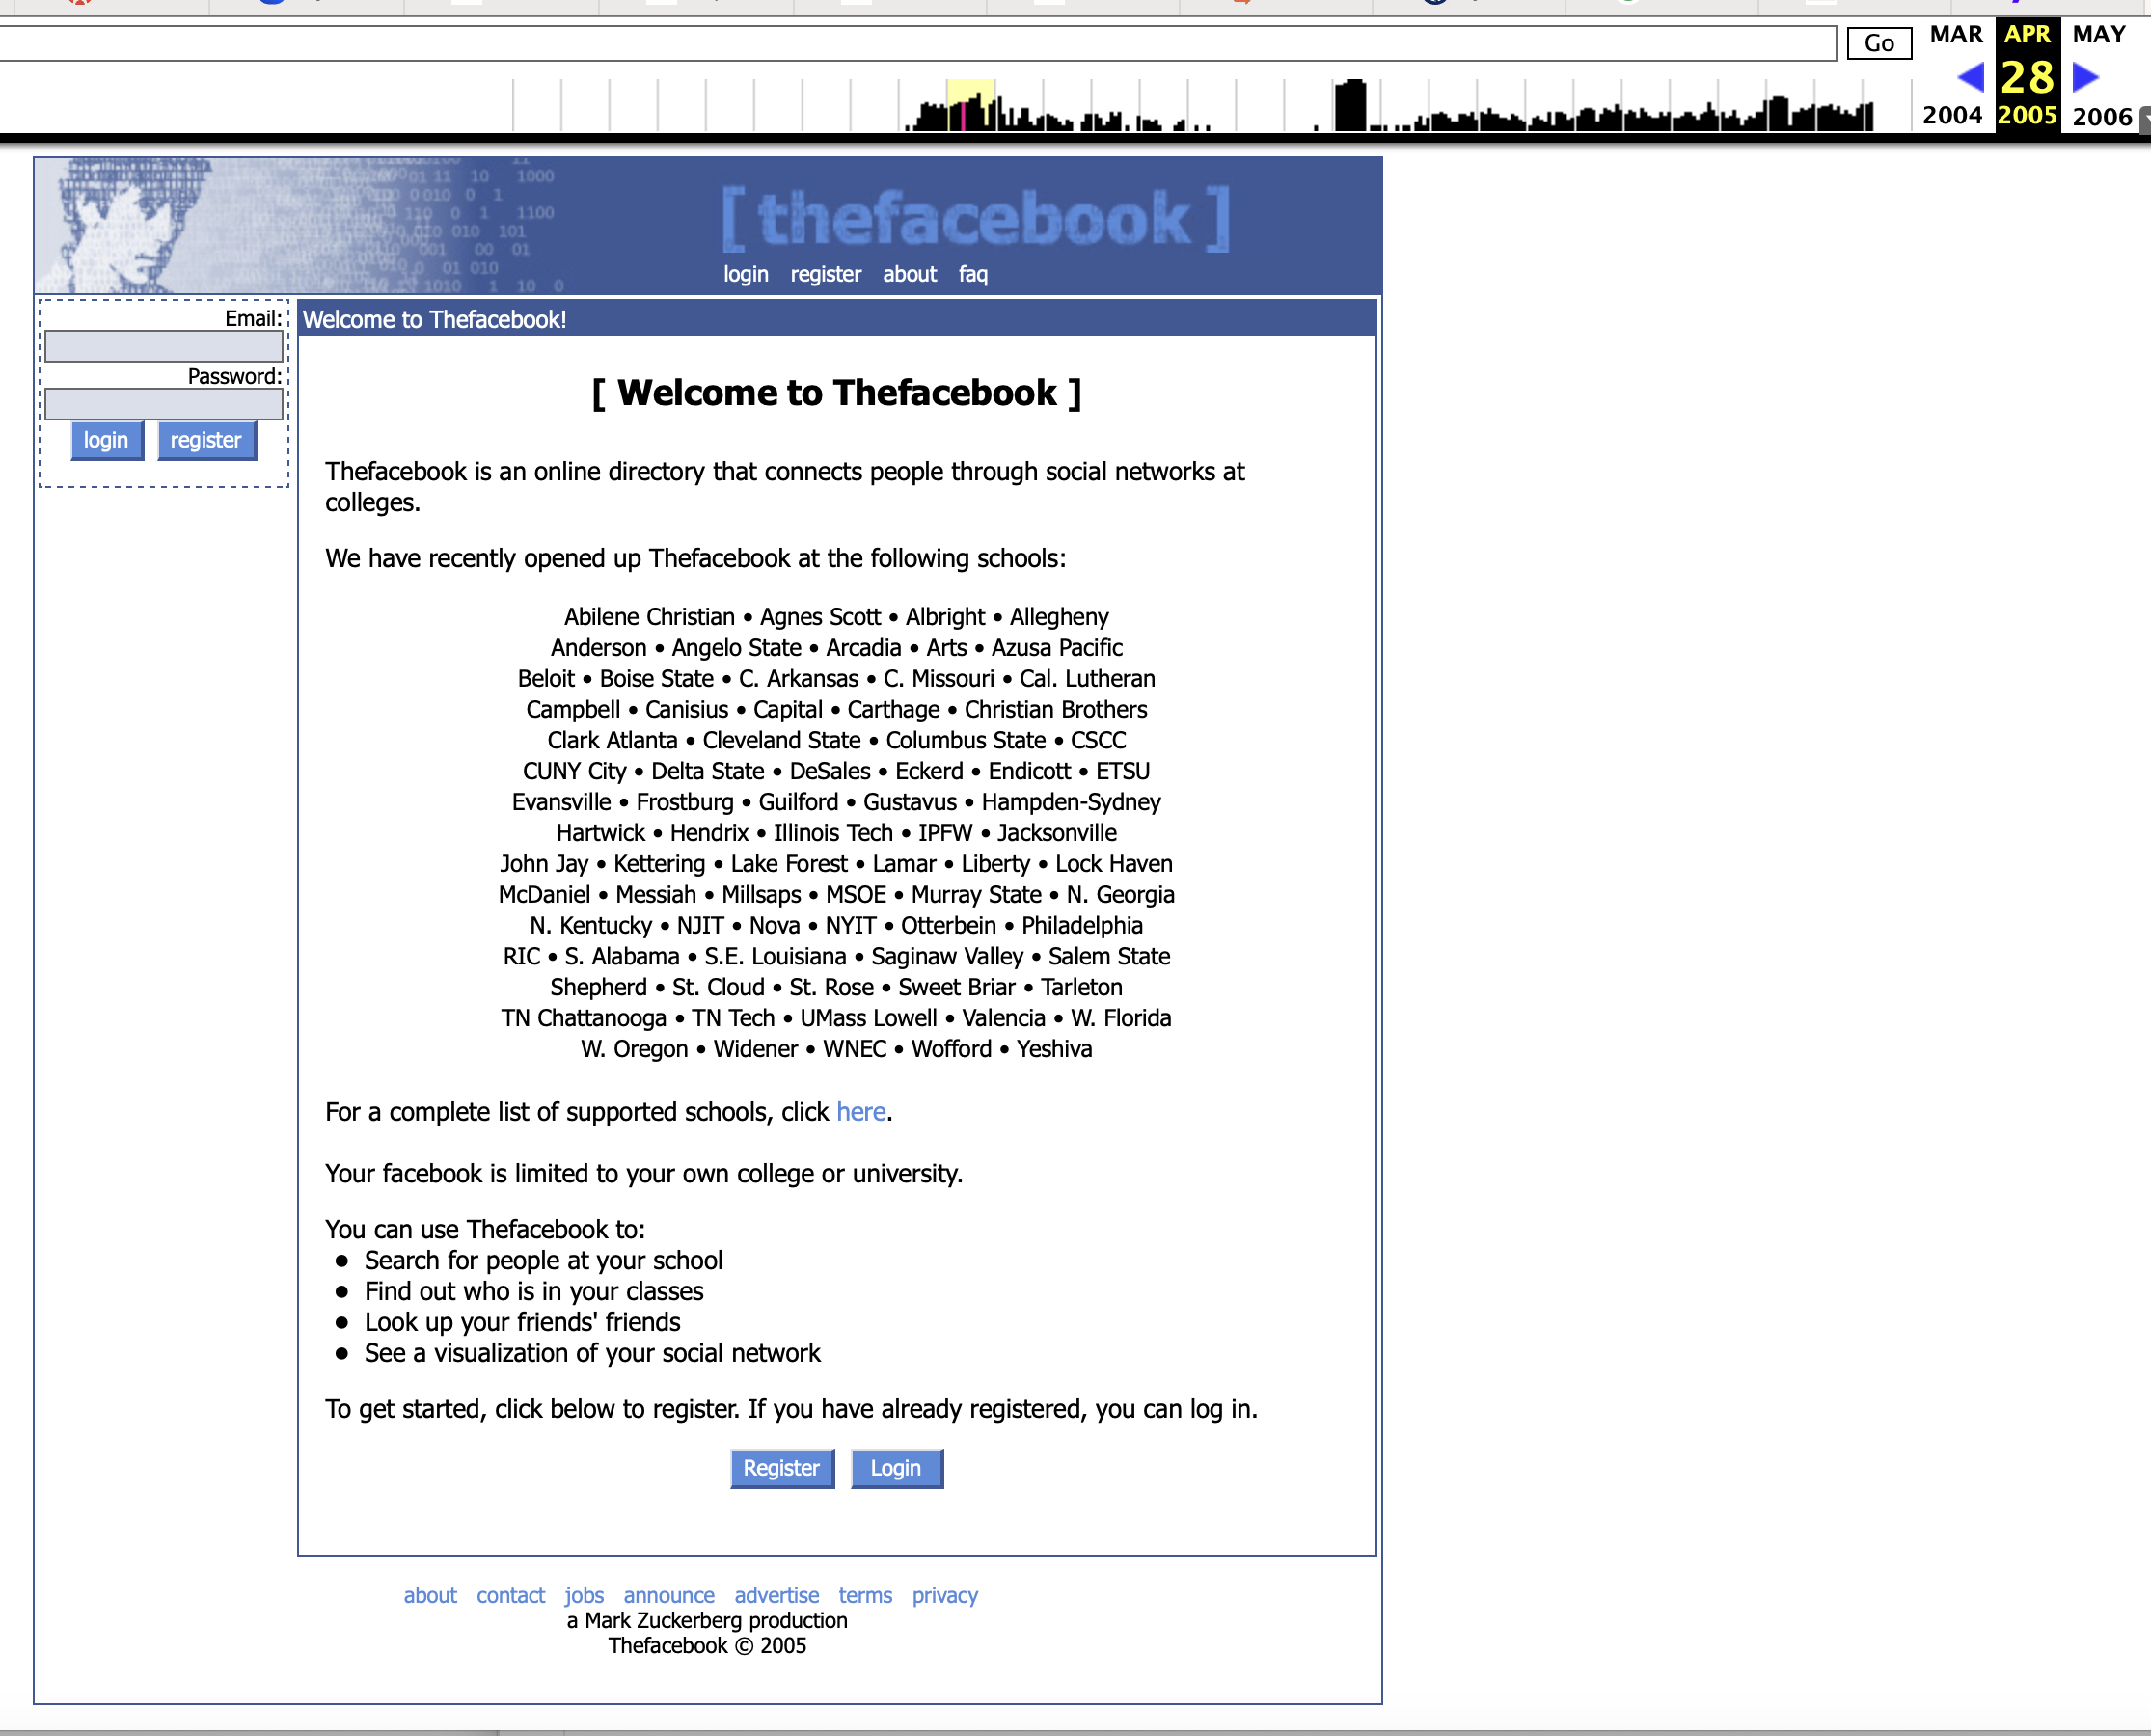
\includegraphics[scale=0.25]{./lecture_includes/wayback4}
\end{center}
\end{frame}

\begin{frame}{Timing Dates}

\begin{itemize}
\item They went through three years, day by day, of daily screenshots on Wayback machine to find when a school appeared on the front page
\item The first time MIT or University of Mississippi appears on the front page, the authors mark that as the date when the school got Facebook
\item But now they need information on mental health outcomes
\item They find it with an old long running repeated cross section survey of college students
\end{itemize}

\end{frame}

\begin{frame}{NCHA survey by ACHA}

\begin{quote}
''Our second main data source consists of more than 430,000 responses to the NCHA survey, a survey administered to college students on a semi-annual basis by the American College Health Association (ACHA). The NCHA survey was developed in 1998 by a team of college health professionals with the purpose of obtaining information from college students about their mental and physical health. Specifically, the NCHA survey inquires about demographics, physical health, \textbf{mental health}, alcohol and drug use, sexual behaviors, and perceptions of these behaviors among one’s peers.''
\end{quote}

\end{frame}

\begin{frame}{No evidence of bite}

\begin{quote}
The NCHA survey does not include any questions on social media use; therefore, it is not possible for us to determine whether a particular survey respondent had a Facebook account.
\end{quote}

\bigskip

This is probably the problem in any study in which your treatment is more or less the first of its kind -- most likely the standard surveys have not yet incorporated the questions into their surveys

\end{frame}

\begin{frame}{Linking Facebook data with NCHA data}

\begin{quote}
In order to protect the privacy of the institutions that participate in the NCHA survey while still allowing us to carry out the analysis, the ACHA kindly agreed to provide us with a customized dataset that includes a variable indicating the semester in which Facebook was rolled out at each college. Specifically, the ACHA adopted the following procedure: (i) merge our dataset containing the Facebook introduction dates to the NCHA dataset; (ii) add a variable listing the semester in which Facebook was rolled out at each college;15 (iii) strip away any information that could allow us to identify colleges (including the specific date in which Facebook was introduced at each college).
\end{quote}

\end{frame}

\begin{frame}{Basic facts about early and late adopters}

\begin{itemize}
\item Colleges in earlier Facebook expansion groups are more selective in terms of test scores, larger, more likely to be on the East Coast, and have more residential undergraduate programs than colleges in later Facebook expansion groups. 

\item Colleges in earlier Facebook expansion groups enroll students from relatively more advantaged economic backgrounds. 

\item Students in colleges that received Facebook relatively earlier have worse baseline mental health outcomes than students attending colleges in later Facebook expansion groups. 

%The baseline differences across Facebook expansion groups may lead one to wonder about the plausibility of the parallel trends assumption in this setting; we address concerns related to parallel trends in Section III.

\end{itemize}

\end{frame}

\begin{frame}{Measurement}

\begin{itemize}
\item The survey data is very rich with a lot of questions about mental health with different scales
\item They create their own combinations of these questions into aggregate indices -- ``index of poor mental health'' where higher numbers mean worse mental health
\item Each outcome survey question is normalized into what is called a ``z-score'' which is interpreted as a fraction of a standard deviation
\item Estimates are ATT parameters -- average effect of Facebook on students at schools that got Facebook
\end{itemize}

\end{frame}


\begin{frame}
\begin{center}
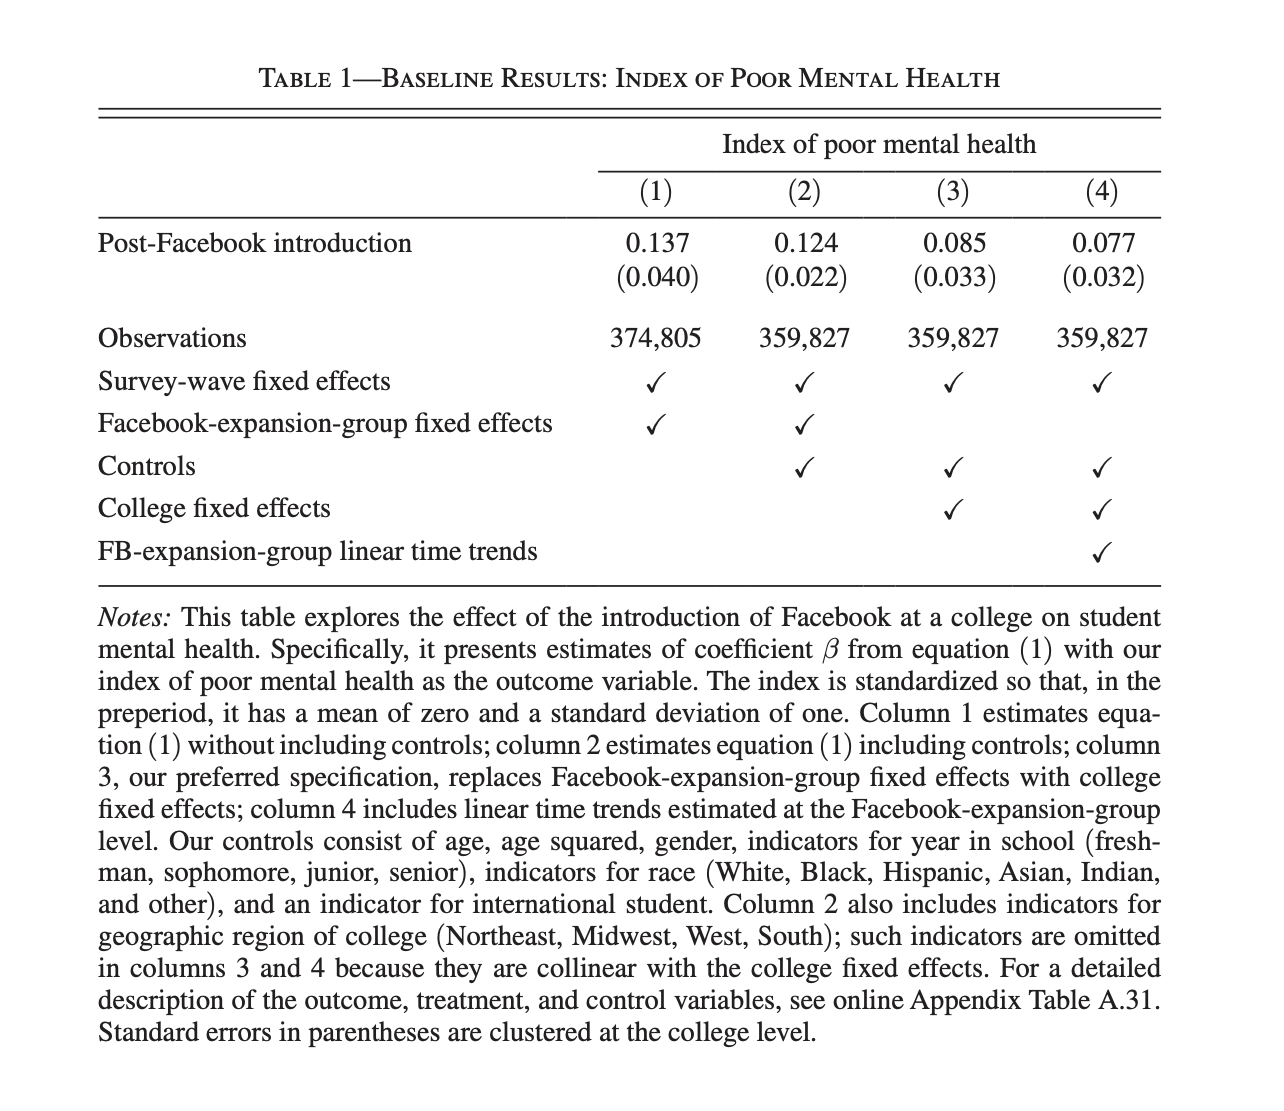
\includegraphics[scale=0.35]{./lecture_includes/facebook_1}
\end{center}
\end{frame}

\begin{frame}
\begin{center}
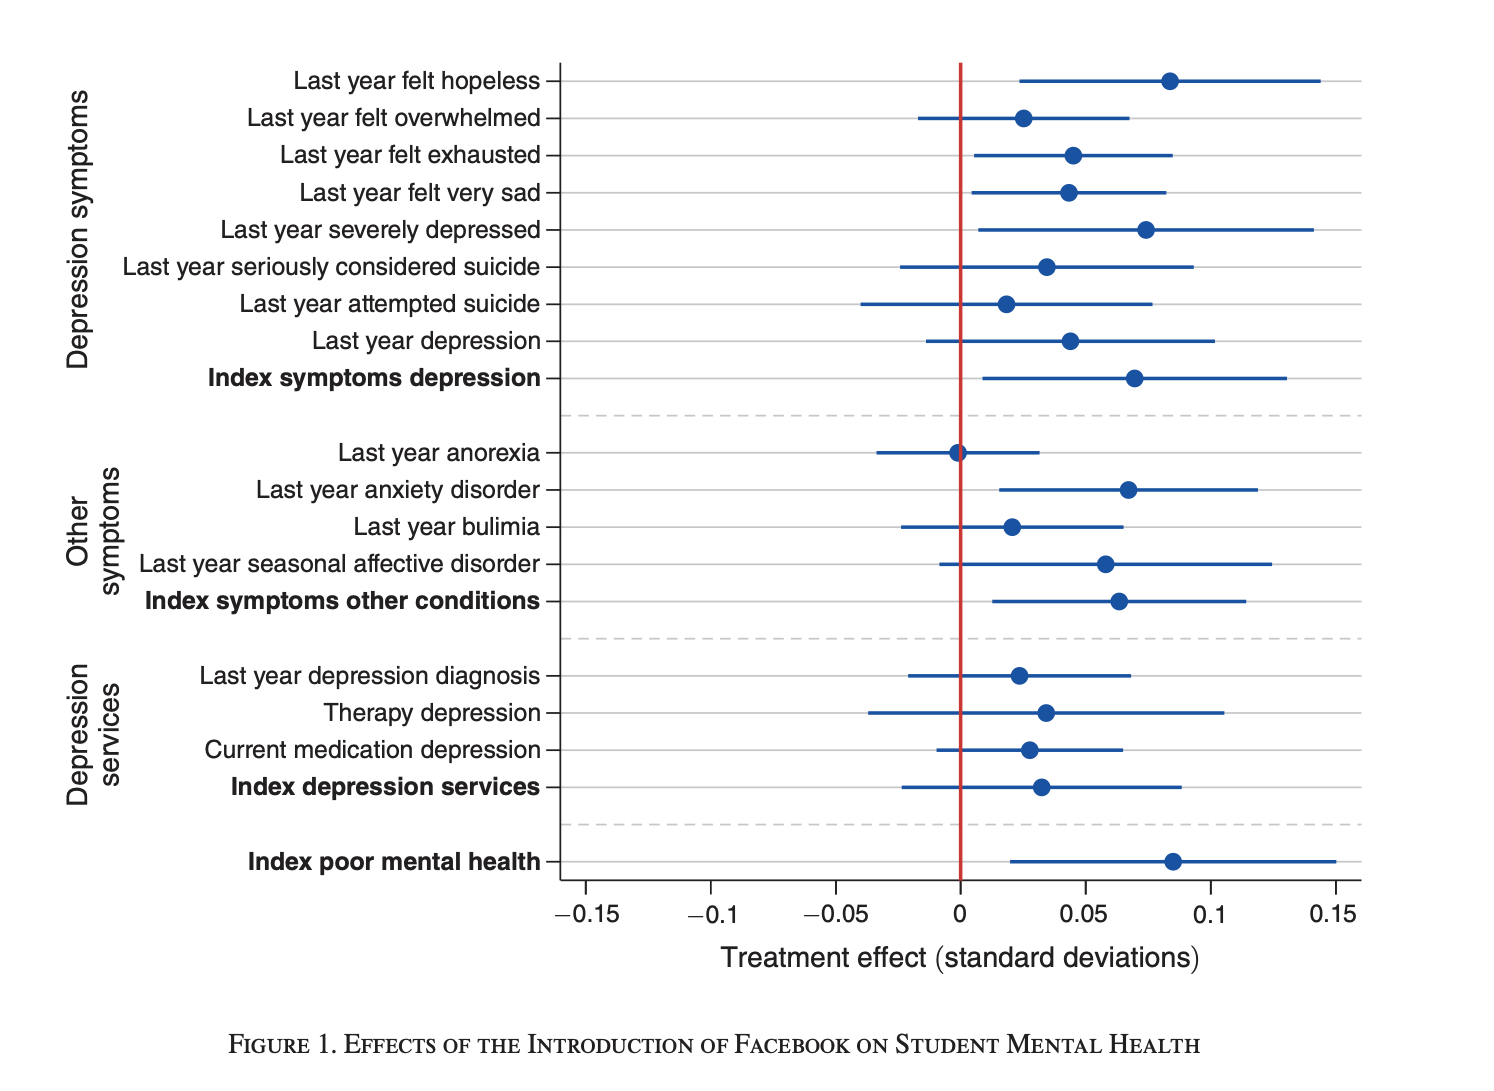
\includegraphics[scale=0.35]{./lecture_includes/facebook_2}
\end{center}
\end{frame}

\begin{frame}{Probably Caused the Acceptance}
\begin{center}
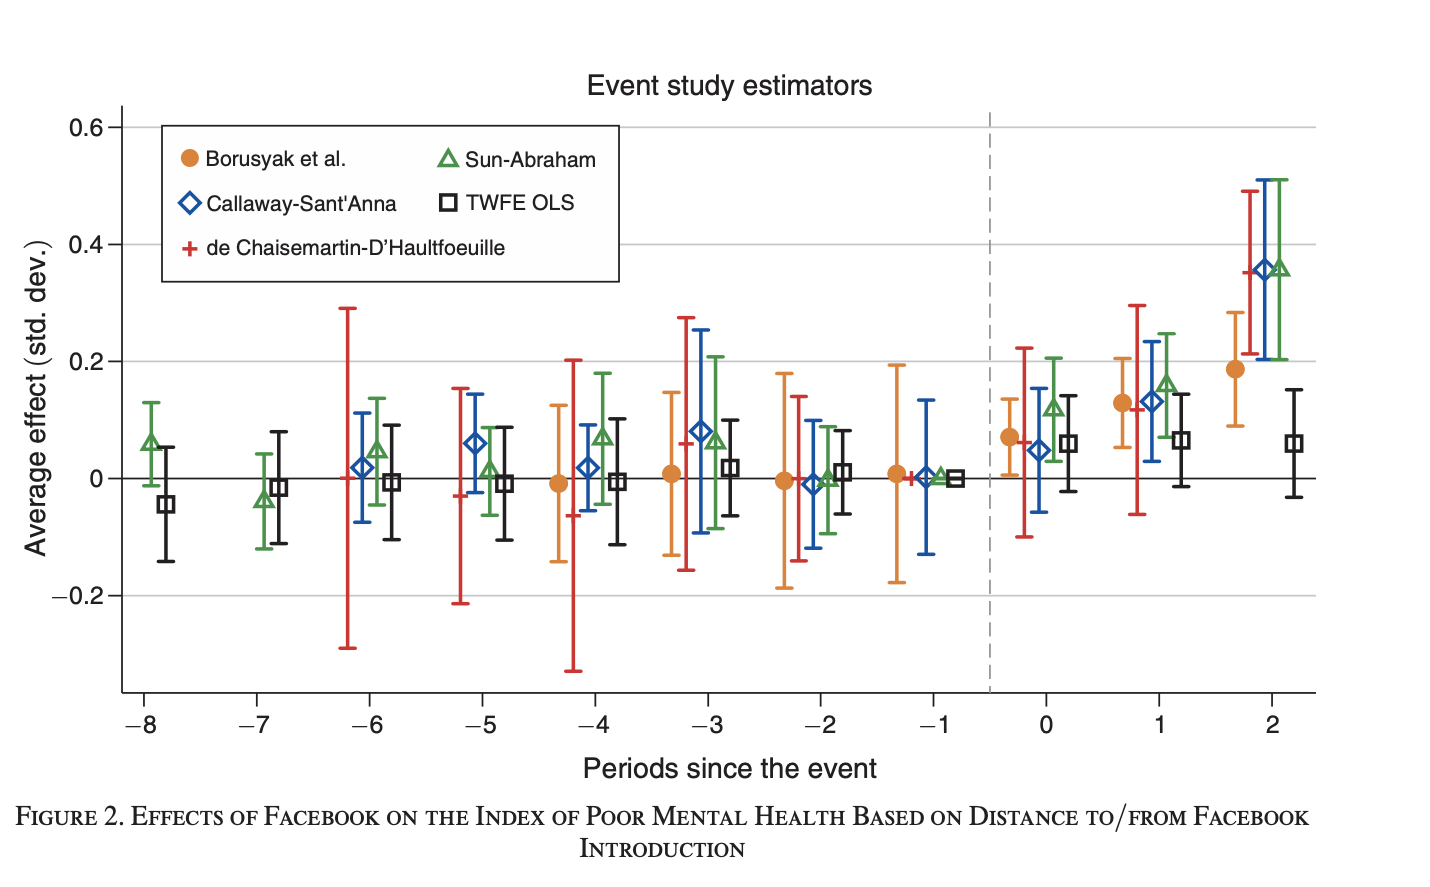
\includegraphics[scale=0.35]{./lecture_includes/facebook_3}
\end{center}
\end{frame}

\begin{frame}{Heterogeneity Analysis and ``Smell Test''}
\begin{center}
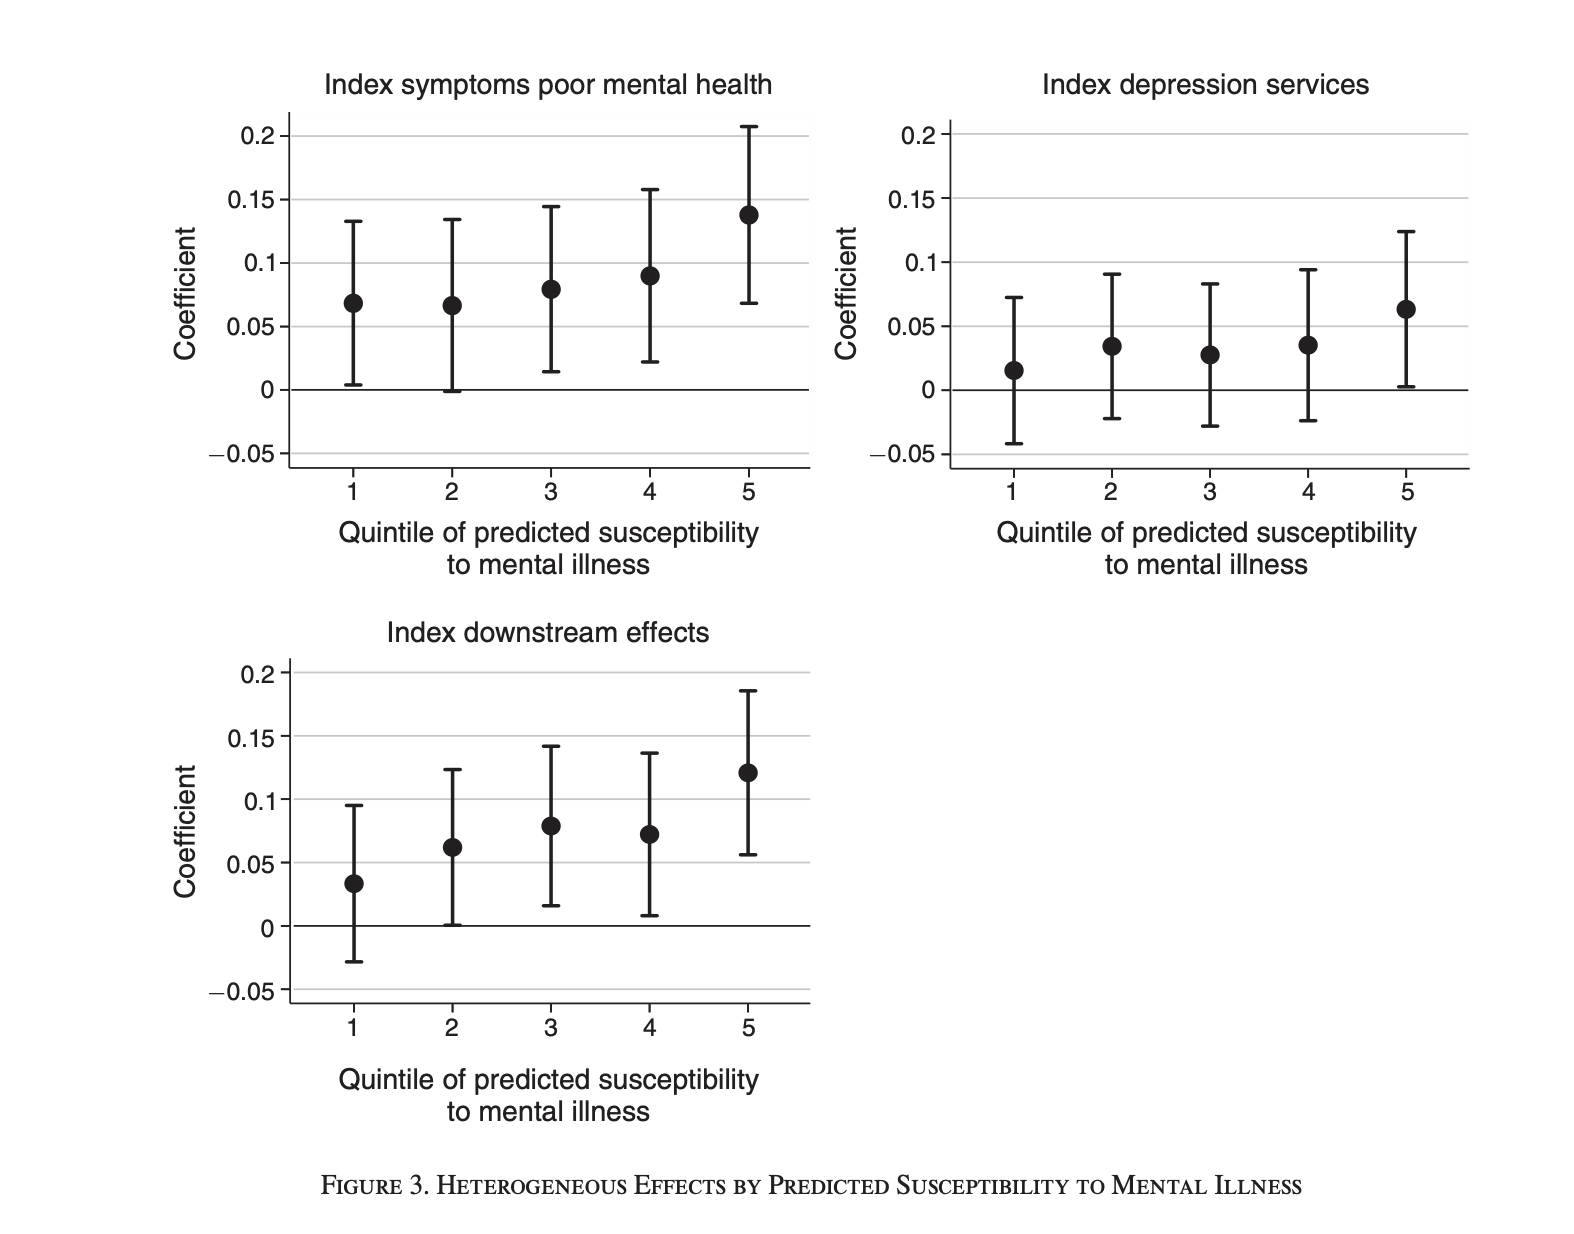
\includegraphics[scale=0.35]{./lecture_includes/facebook_4}
\end{center}
\end{frame}

\begin{frame}{Exposure Worsens}
\begin{center}
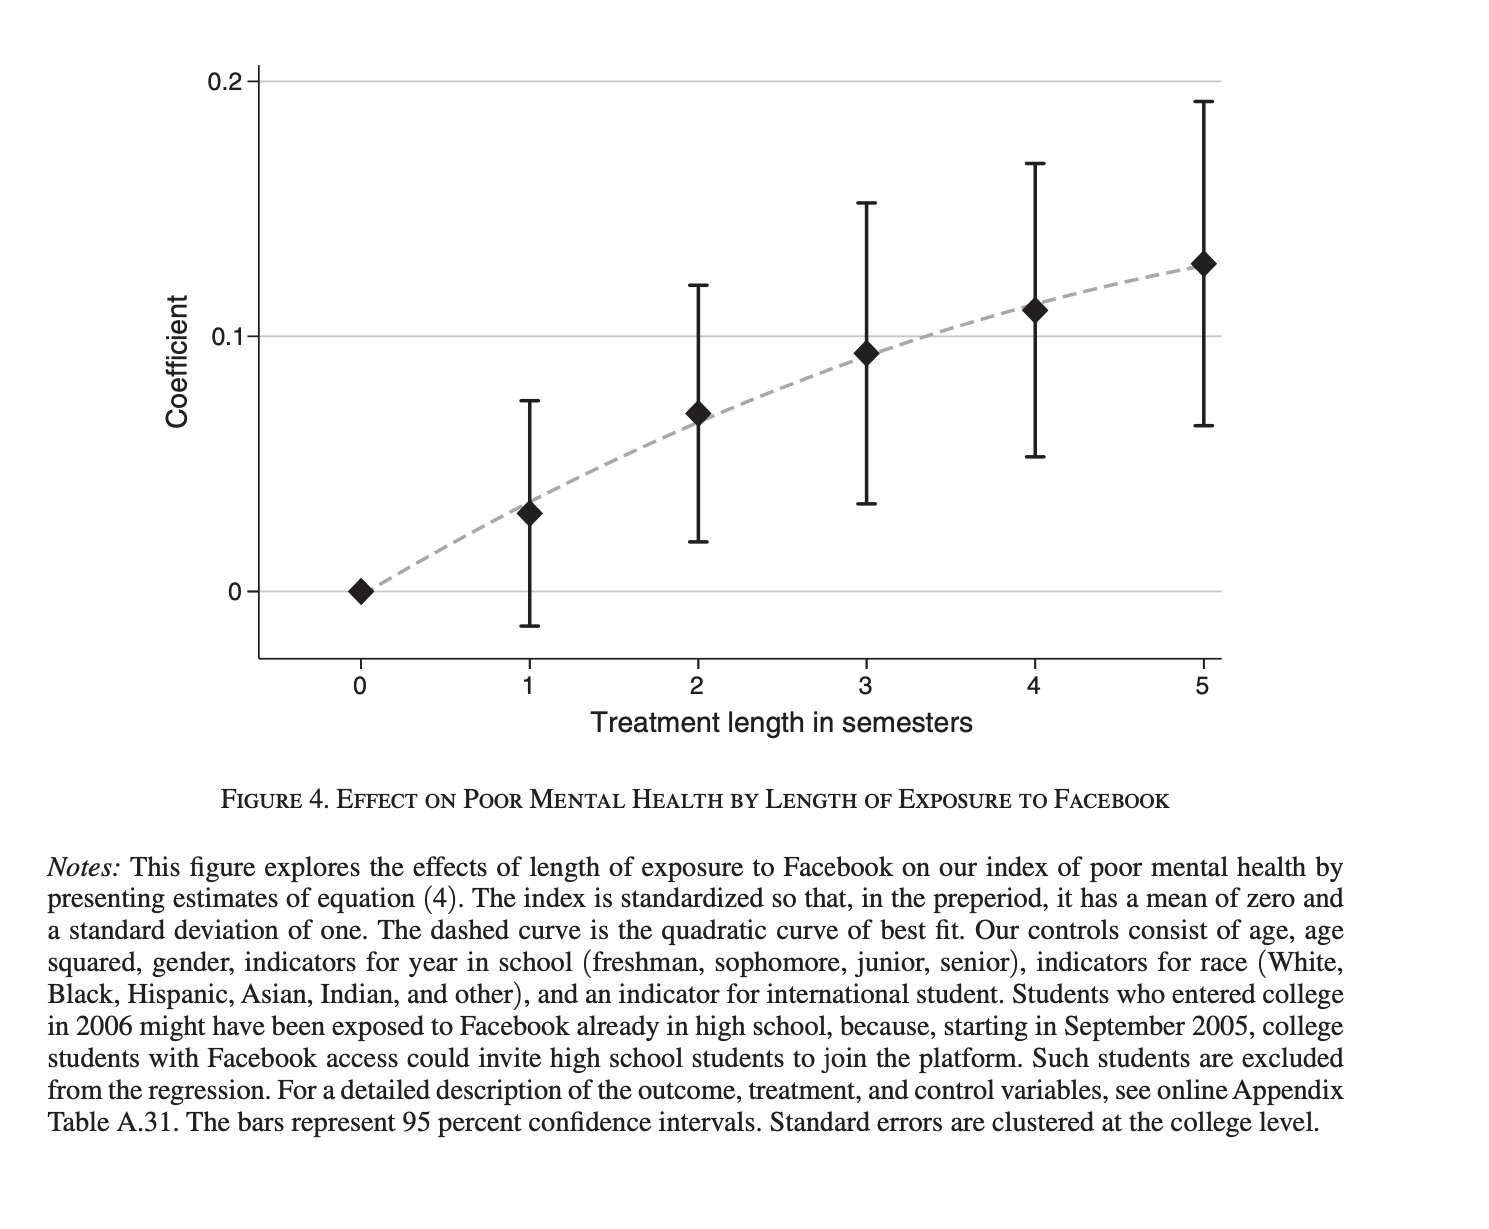
\includegraphics[scale=0.35]{./lecture_includes/facebook_5}
\end{center}
\end{frame}

\begin{frame}{Academic Effects}
\begin{center}
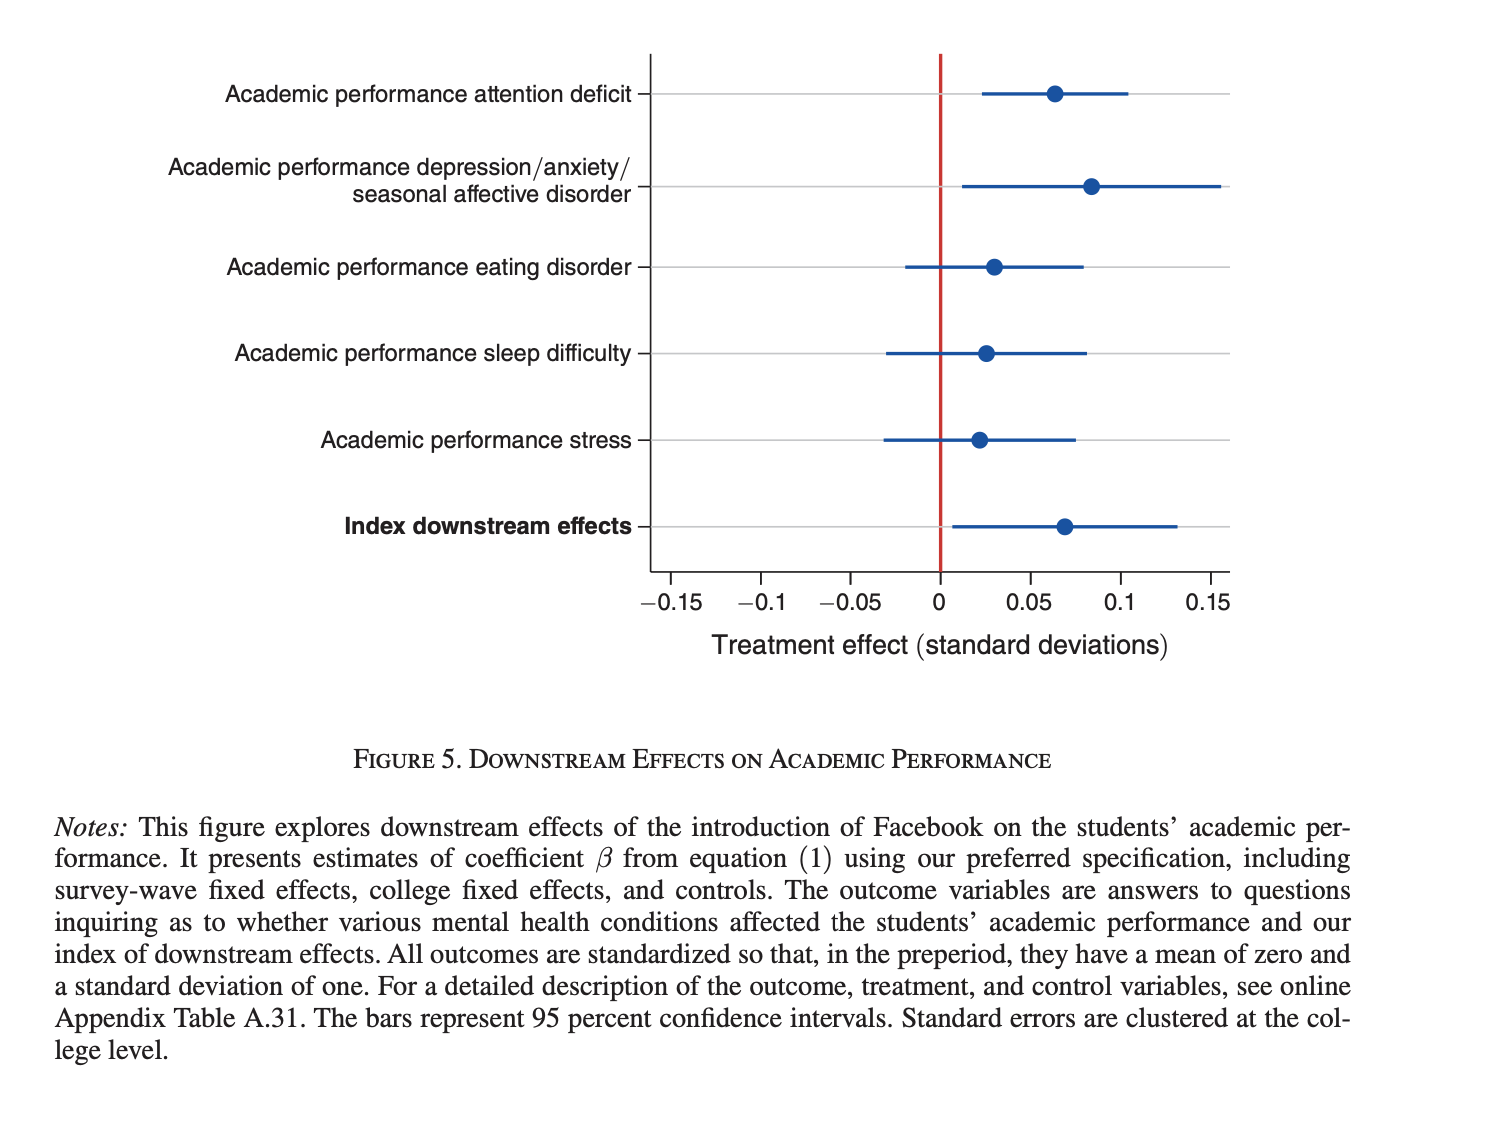
\includegraphics[scale=0.35]{./lecture_includes/facebook_6}
\end{center}
\end{frame}

\begin{frame}{Mechanisms}
\begin{center}
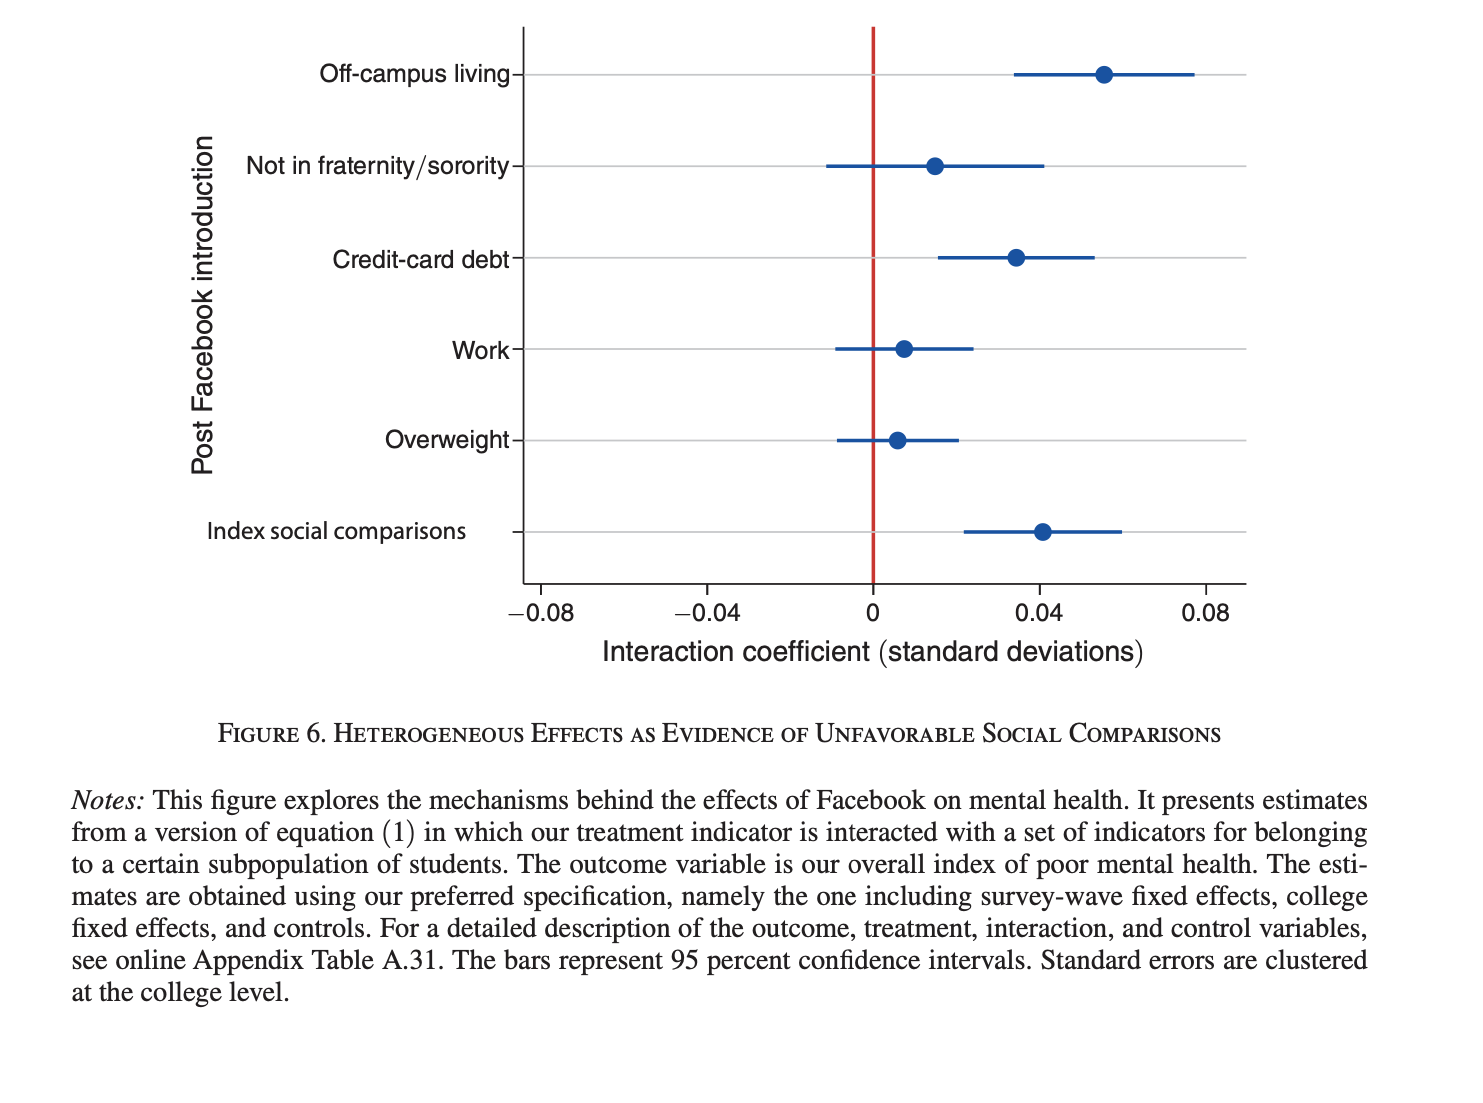
\includegraphics[scale=0.35]{./lecture_includes/facebook_7}
\end{center}
\end{frame}

\begin{frame}{Questions and Comments}

\begin{itemize}
\item Mark Zuckerberg quote: ``the existing body of scientific work has not shown a causal link between using social media and young people having worse mental health outcomes'' -- What is your reaction to his claim?
\item What is your reaction to this study's evidence?  
\item Which parts of this study do you think is more memorable and more convincing and why?
\item How might you replicate this study yourself?

\end{itemize}

\end{frame}


\subsection{Generative AI and Worker Productivity}

\begin{frame}{Working Paper on ChatBot}
\begin{center}
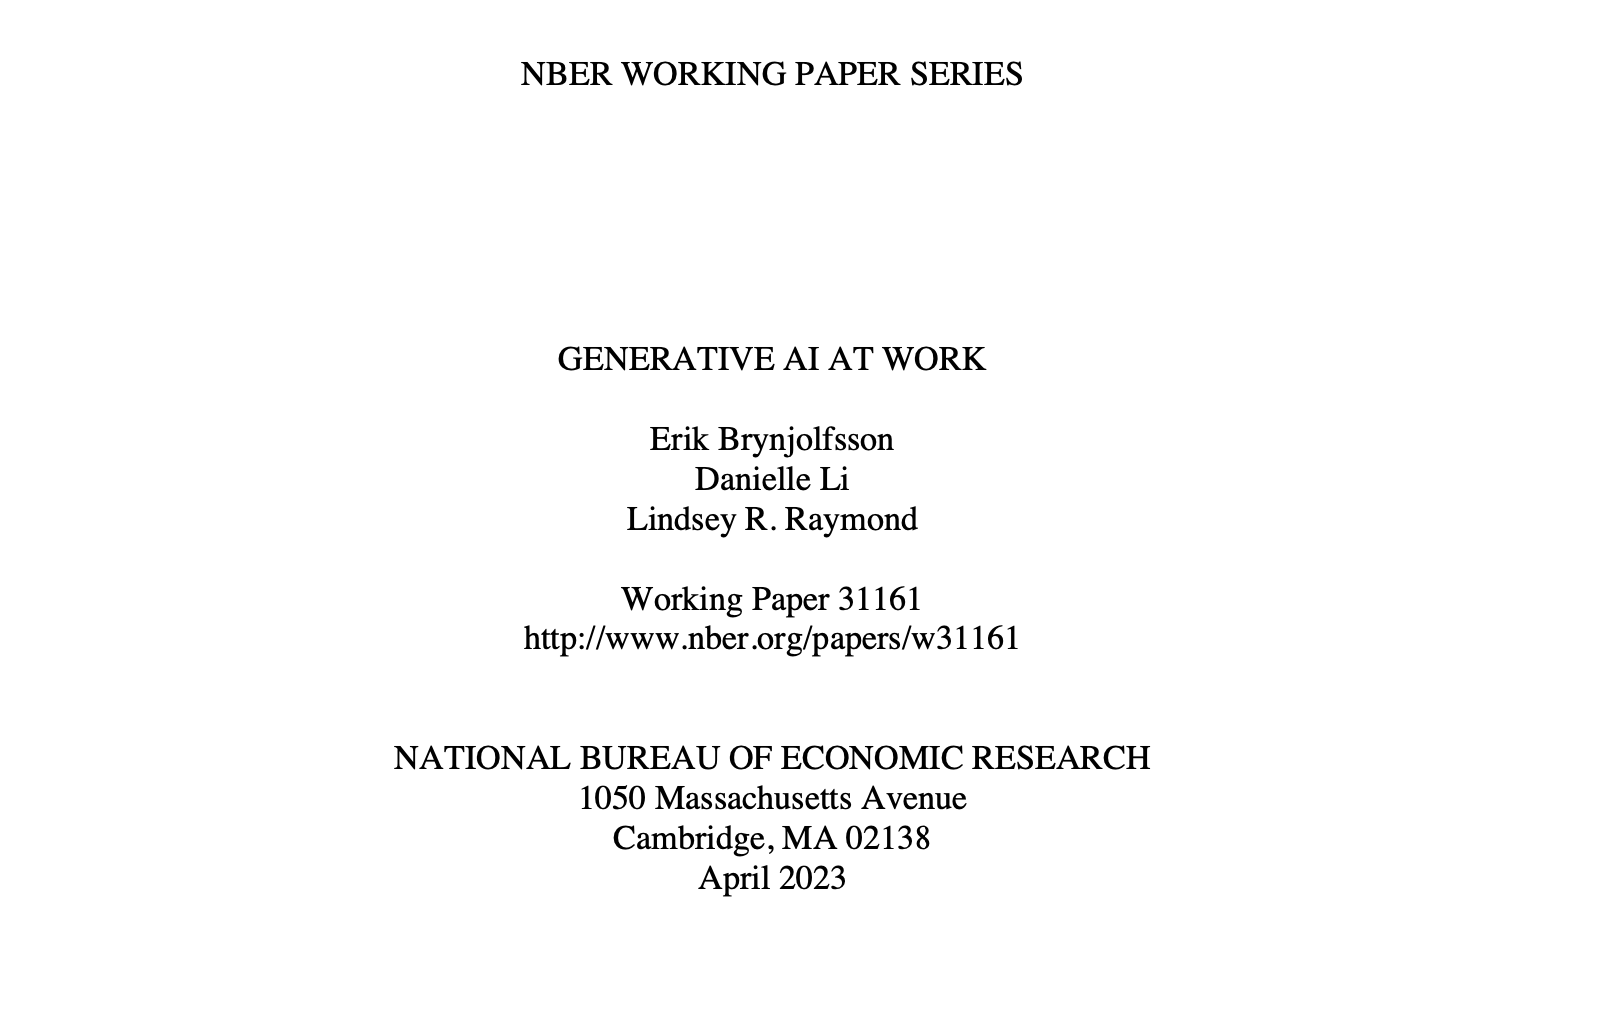
\includegraphics[scale=0.35]{./lecture_includes/brynn}
\end{center}
\end{frame}



\begin{frame}{Chatbots and Workers}

\begin{itemize}

\item An unnamed firm released gradually a generative AI-based conversational assistant chatbot to its  5,179 customer support agents 
\item These chatbots provided assistance in handling complaints
\item Very stressful job as the only time customers reached out was when they were very upset
\item It isn't a randomized experiment so they're going to estimate the effect of the adoption of the chatbot using difference-in-differences

\end{itemize}

\end{frame}

\begin{frame}{Outcomes and Pictures}

\begin{itemize}

\item Main focus is on various measures of customer support agents handling of calls, which is the proxy for their productivity
\item But they also focus on high and low skill workers (heterogeneity like before)
\item Authors are going to present evidence almost entirely using event study graphs
\item They also present regression tables, but the event study graphs are very powerful

\end{itemize}

\end{frame}




\begin{frame}{Example of ChatBot}
\begin{center}
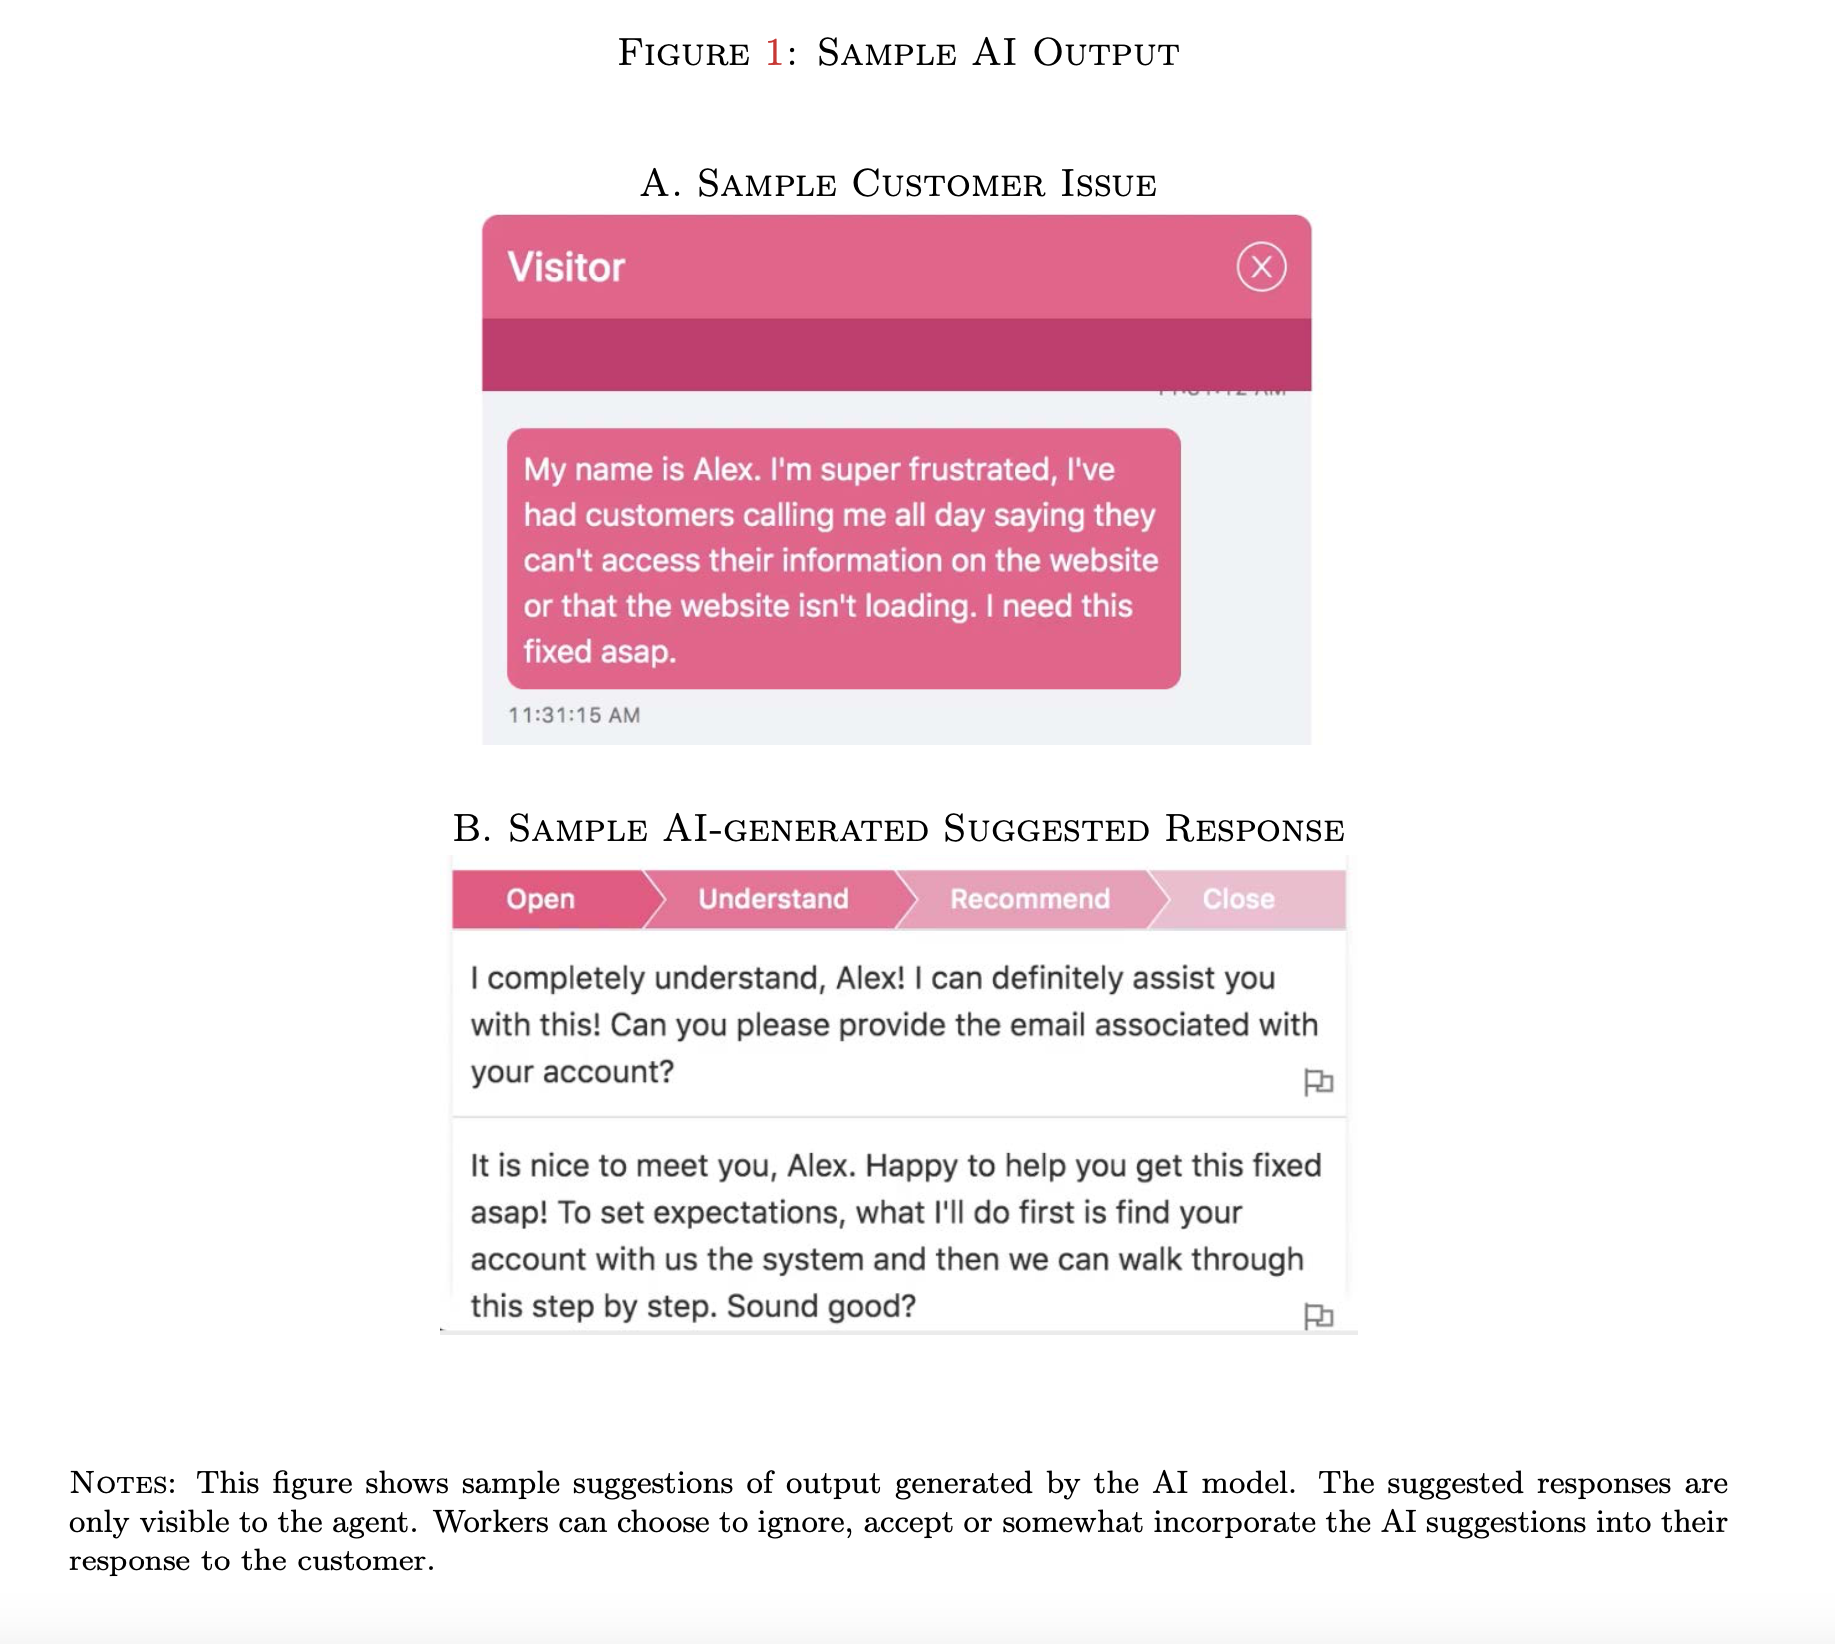
\includegraphics[scale=0.35]{./lecture_includes/brynn1}
\end{center}
\end{frame}


\begin{frame}{Rollout}
\begin{center}
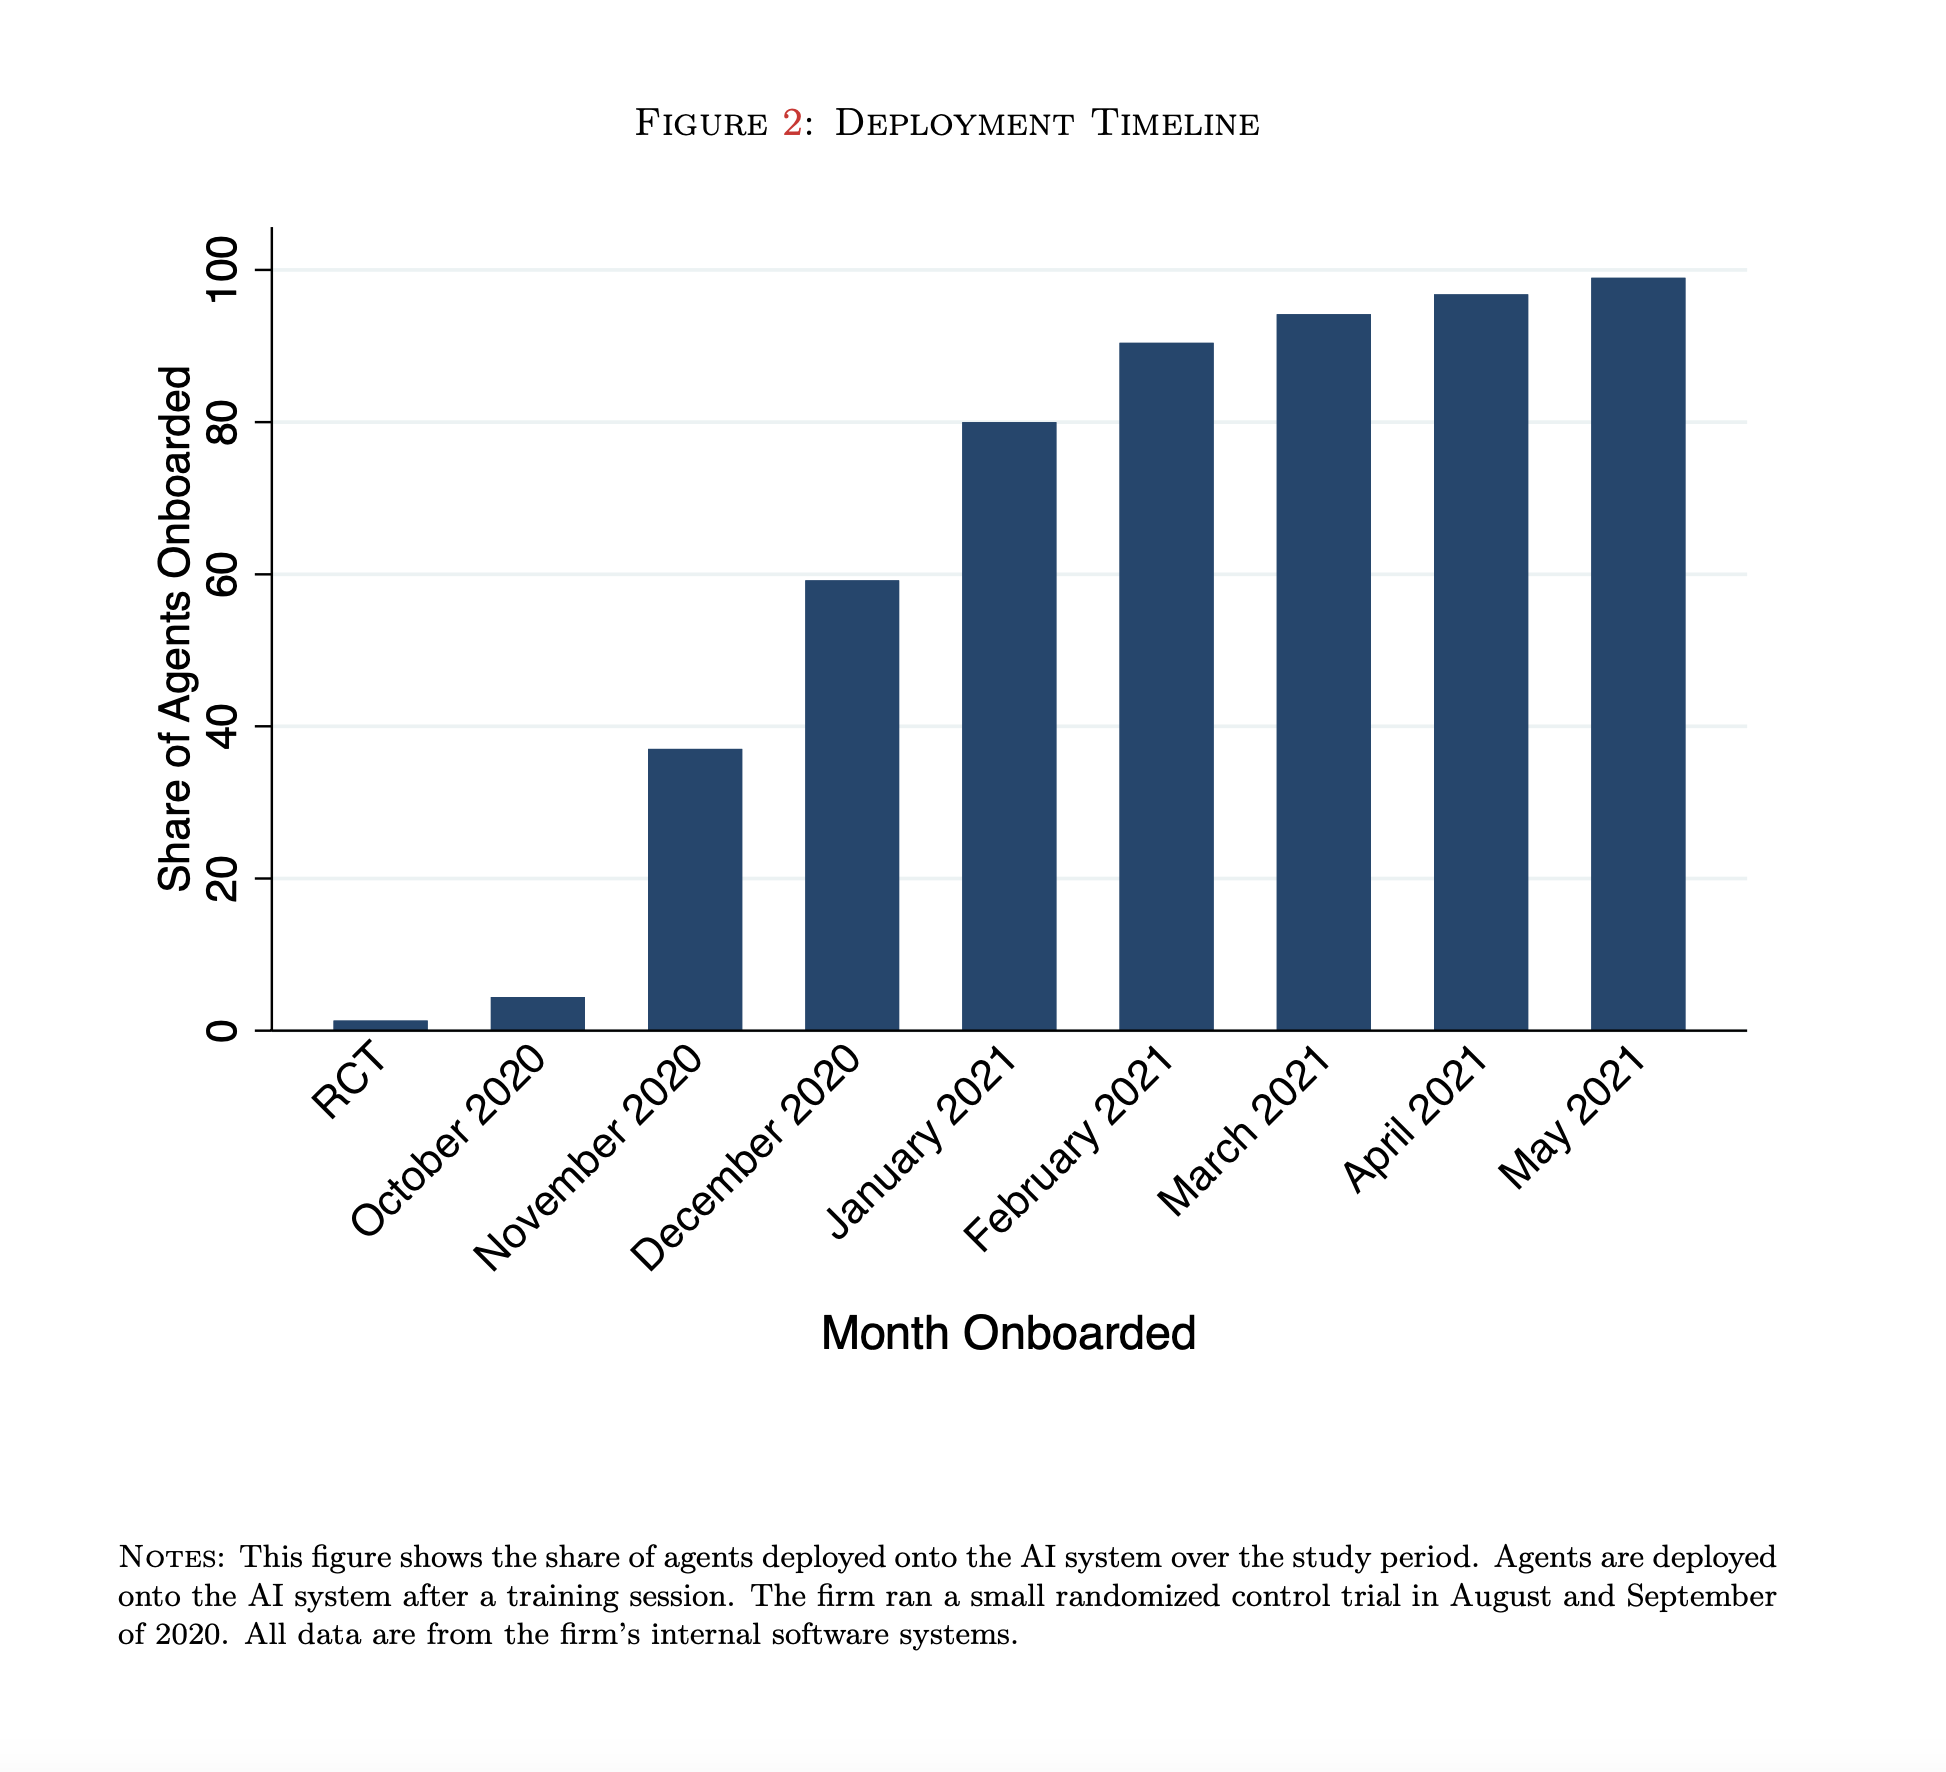
\includegraphics[scale=0.35]{./lecture_includes/brynn2}
\end{center}
\end{frame}


\begin{frame}{All the diff-in-diffs vs Sun and Abraham}
\begin{multicols}{2}

\begin{figure}
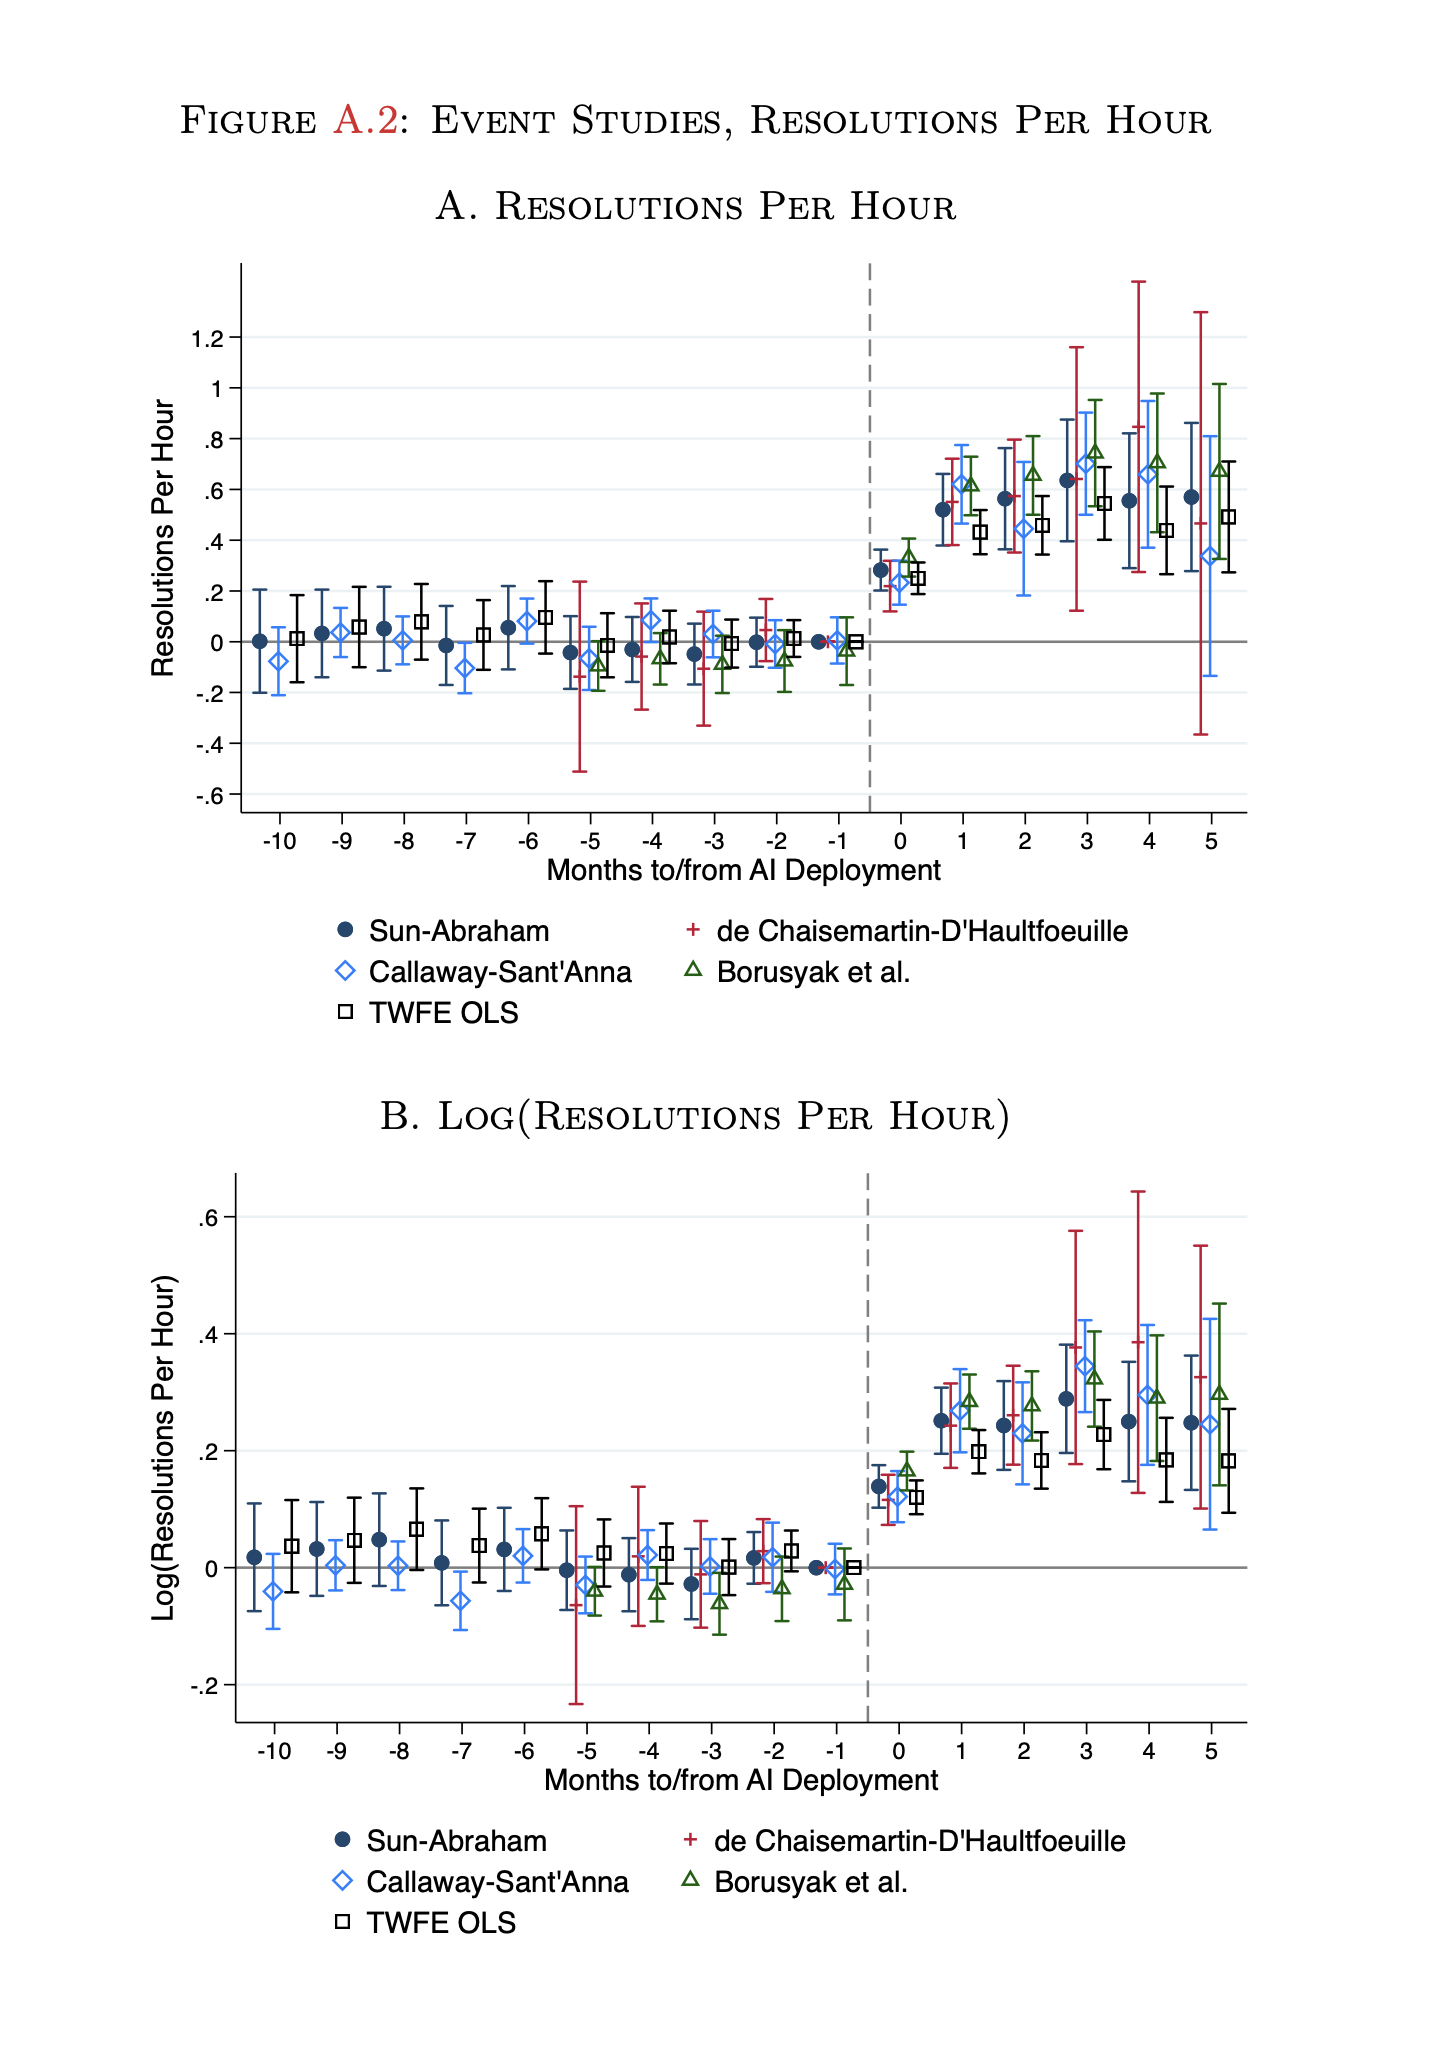
\includegraphics[width=0.95\linewidth, keepaspectratio]{./lecture_includes/genai_did}
\end{figure}

\begin{figure}
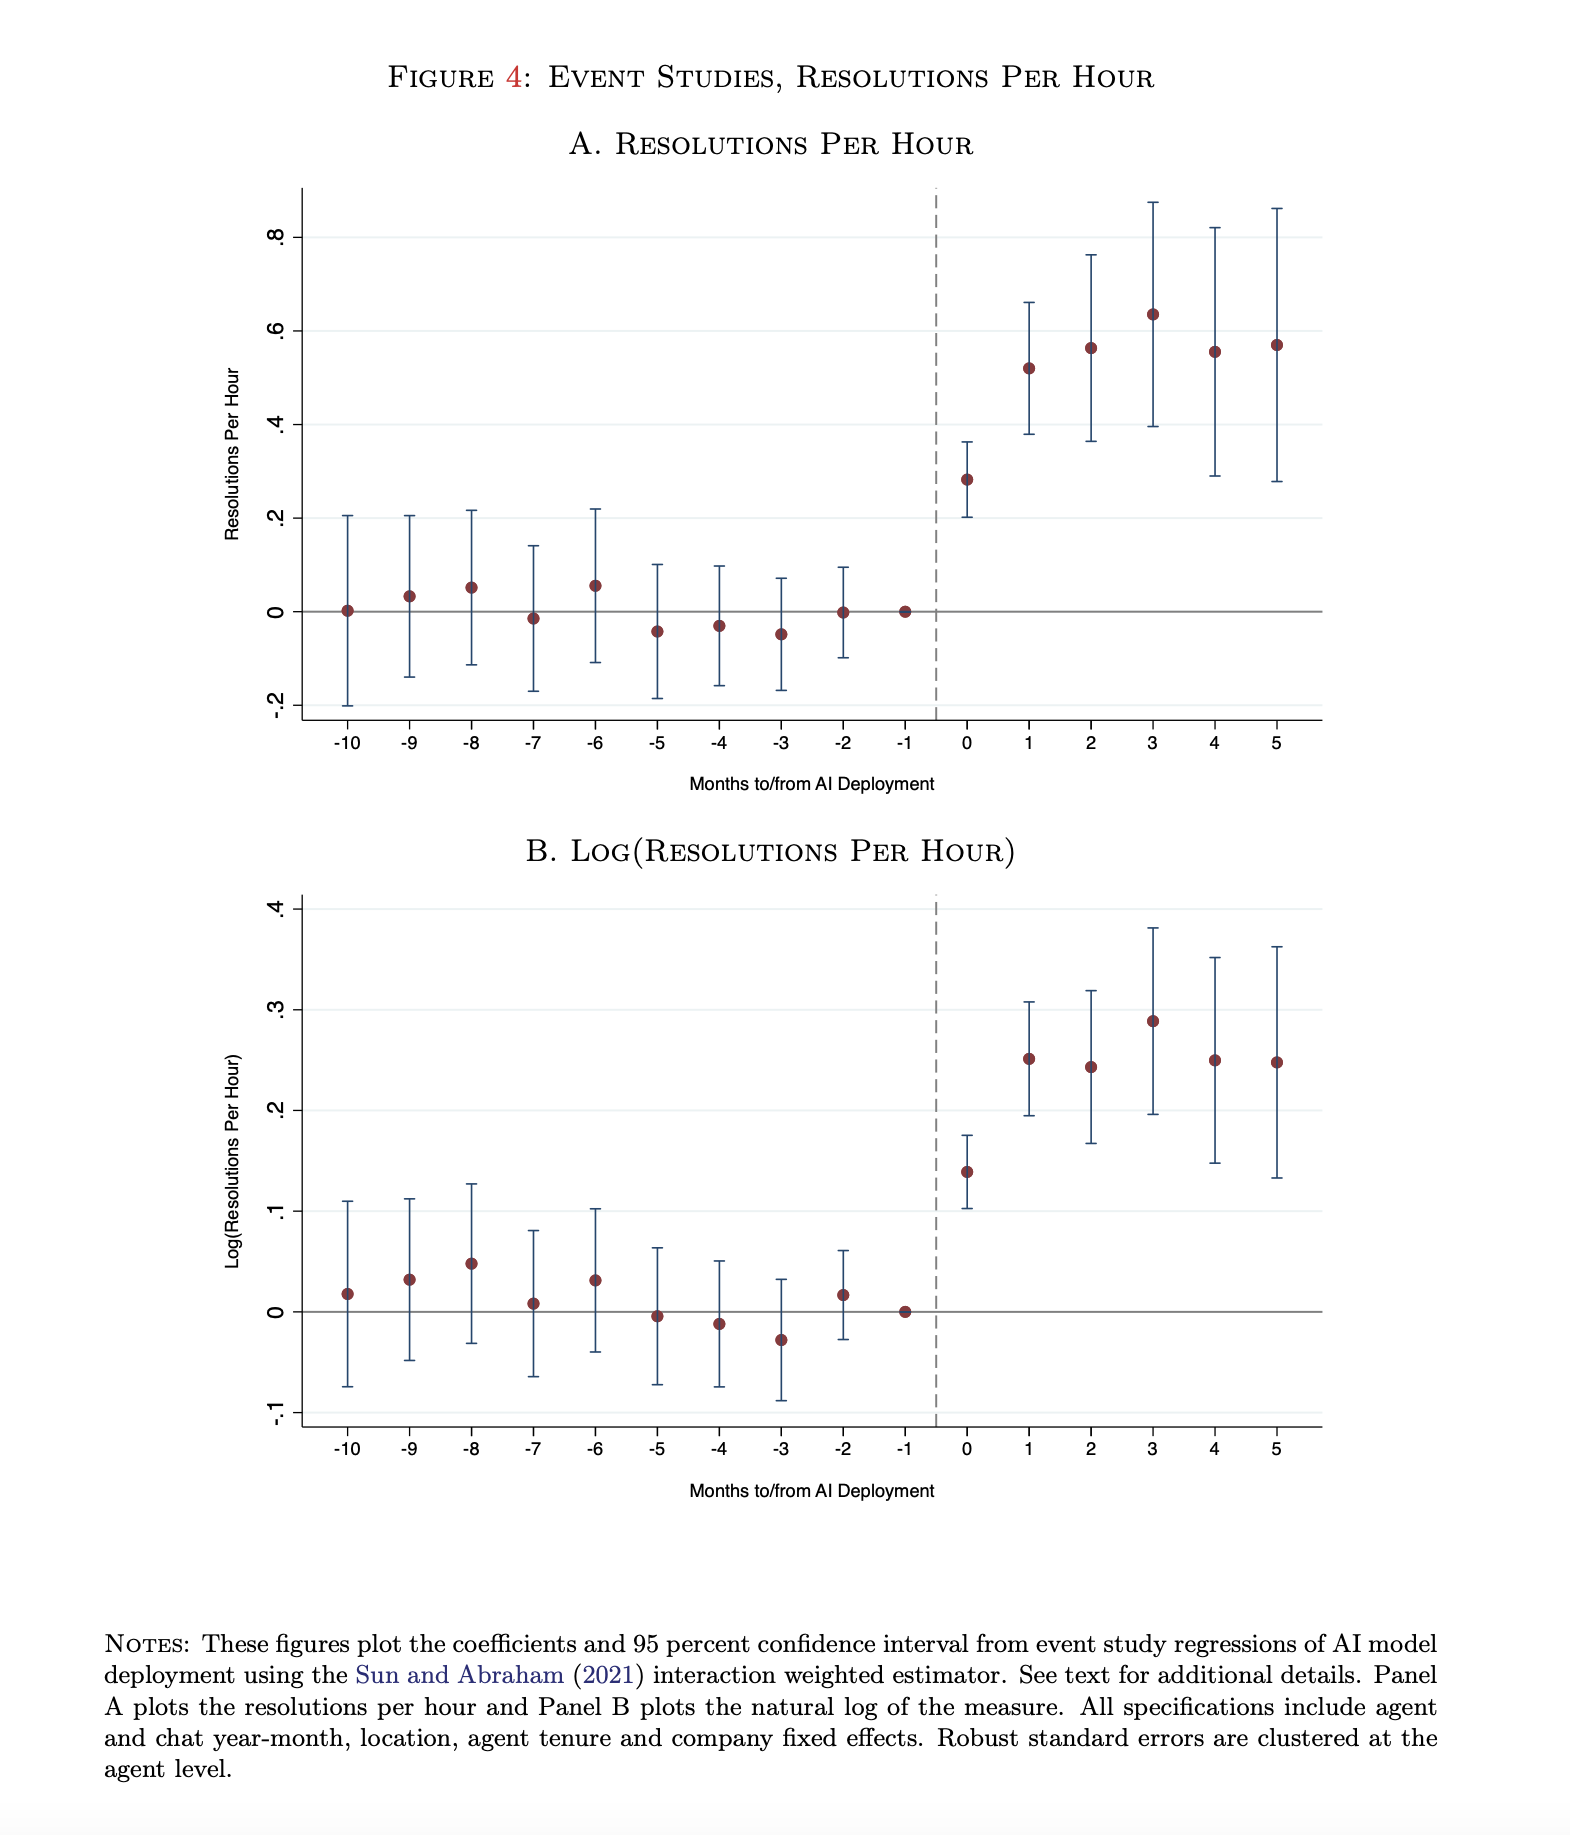
\includegraphics[scale=0.22]{./lecture_includes/brynn3}
\end{figure}

\end{multicols}
\end{frame}

\begin{frame}{Comments}

\begin{itemize}

\item They showed what is becoming standard ``all the diff in diffs''
\item But then they stick with Sun and Abraham for all analysis (all the diff in diffs is an appendix figure)
\item They also produce a table in the appendix of their simple ATTs for everything
\item Contrast this with the Facebook paper which showed TWFE \emph{even though TWFE was biased}

\end{itemize}

\end{frame}


\begin{frame}{Additional Outcomes}
\begin{center}
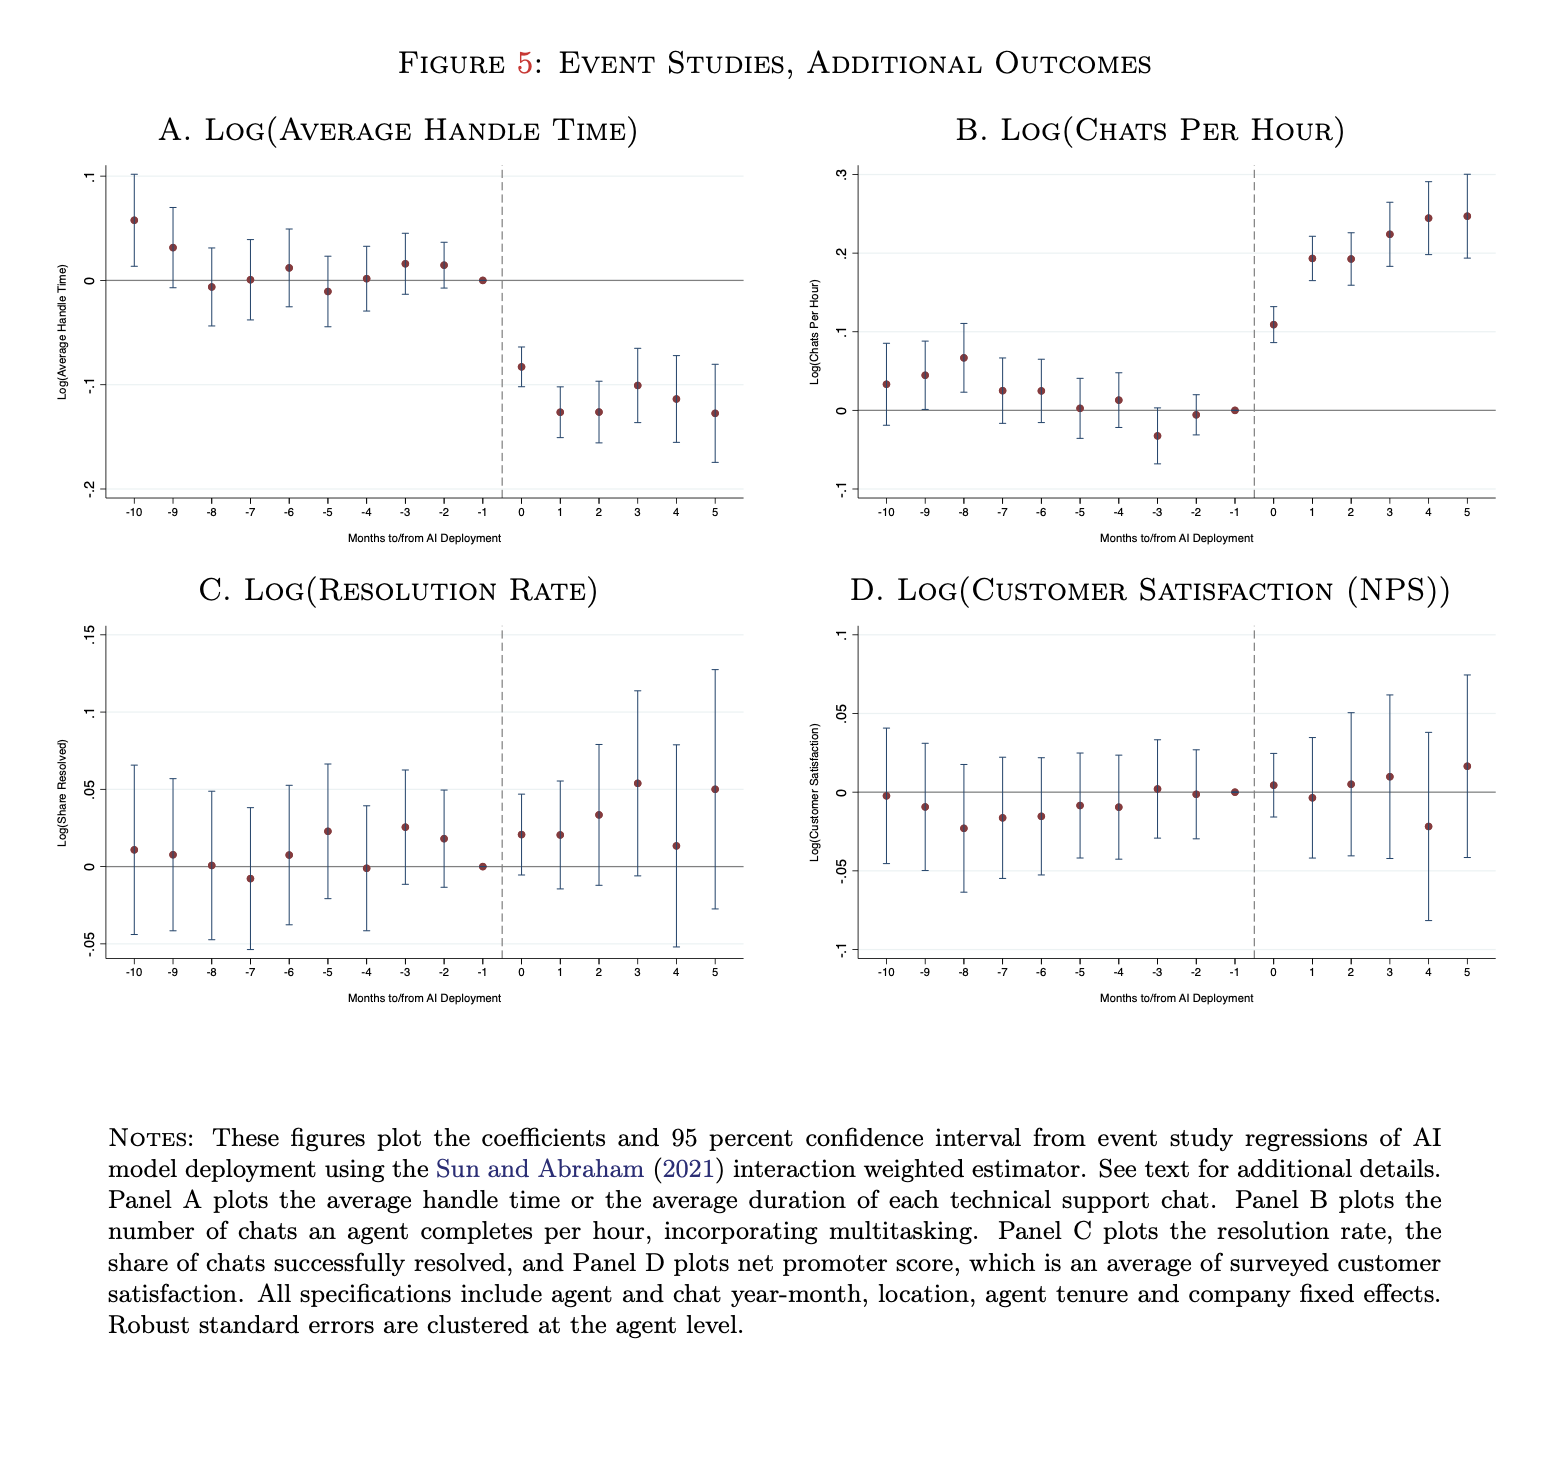
\includegraphics[scale=0.35]{./lecture_includes/brynn4}
\end{center}
\end{frame}

\begin{frame}{Heterogeneity by Skill}
\begin{center}
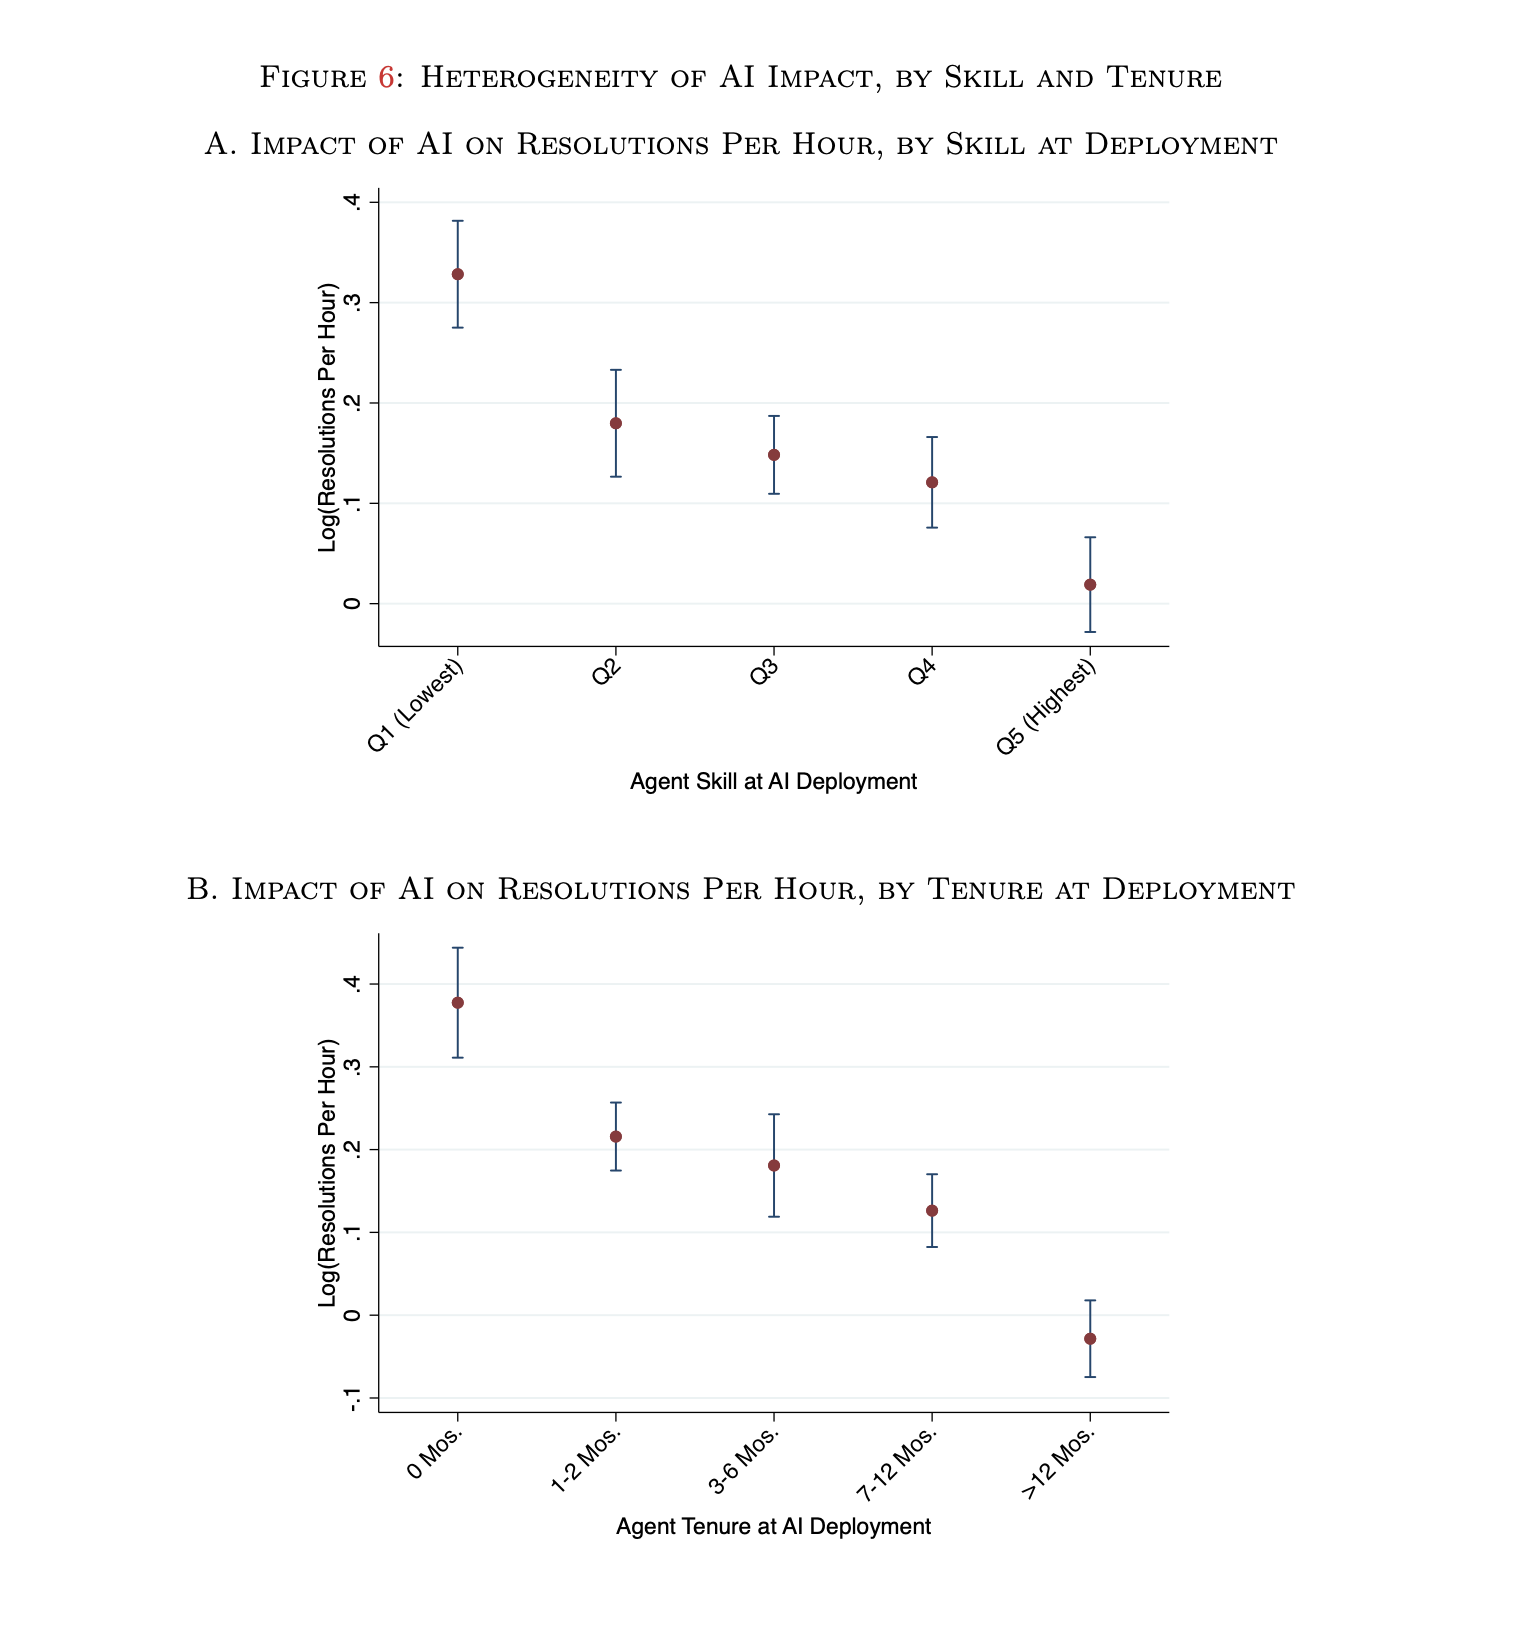
\includegraphics[scale=0.25]{./lecture_includes/brynn5}
\end{center}
\end{frame}


\begin{frame}{Heterogeneity by Skill}
\begin{center}
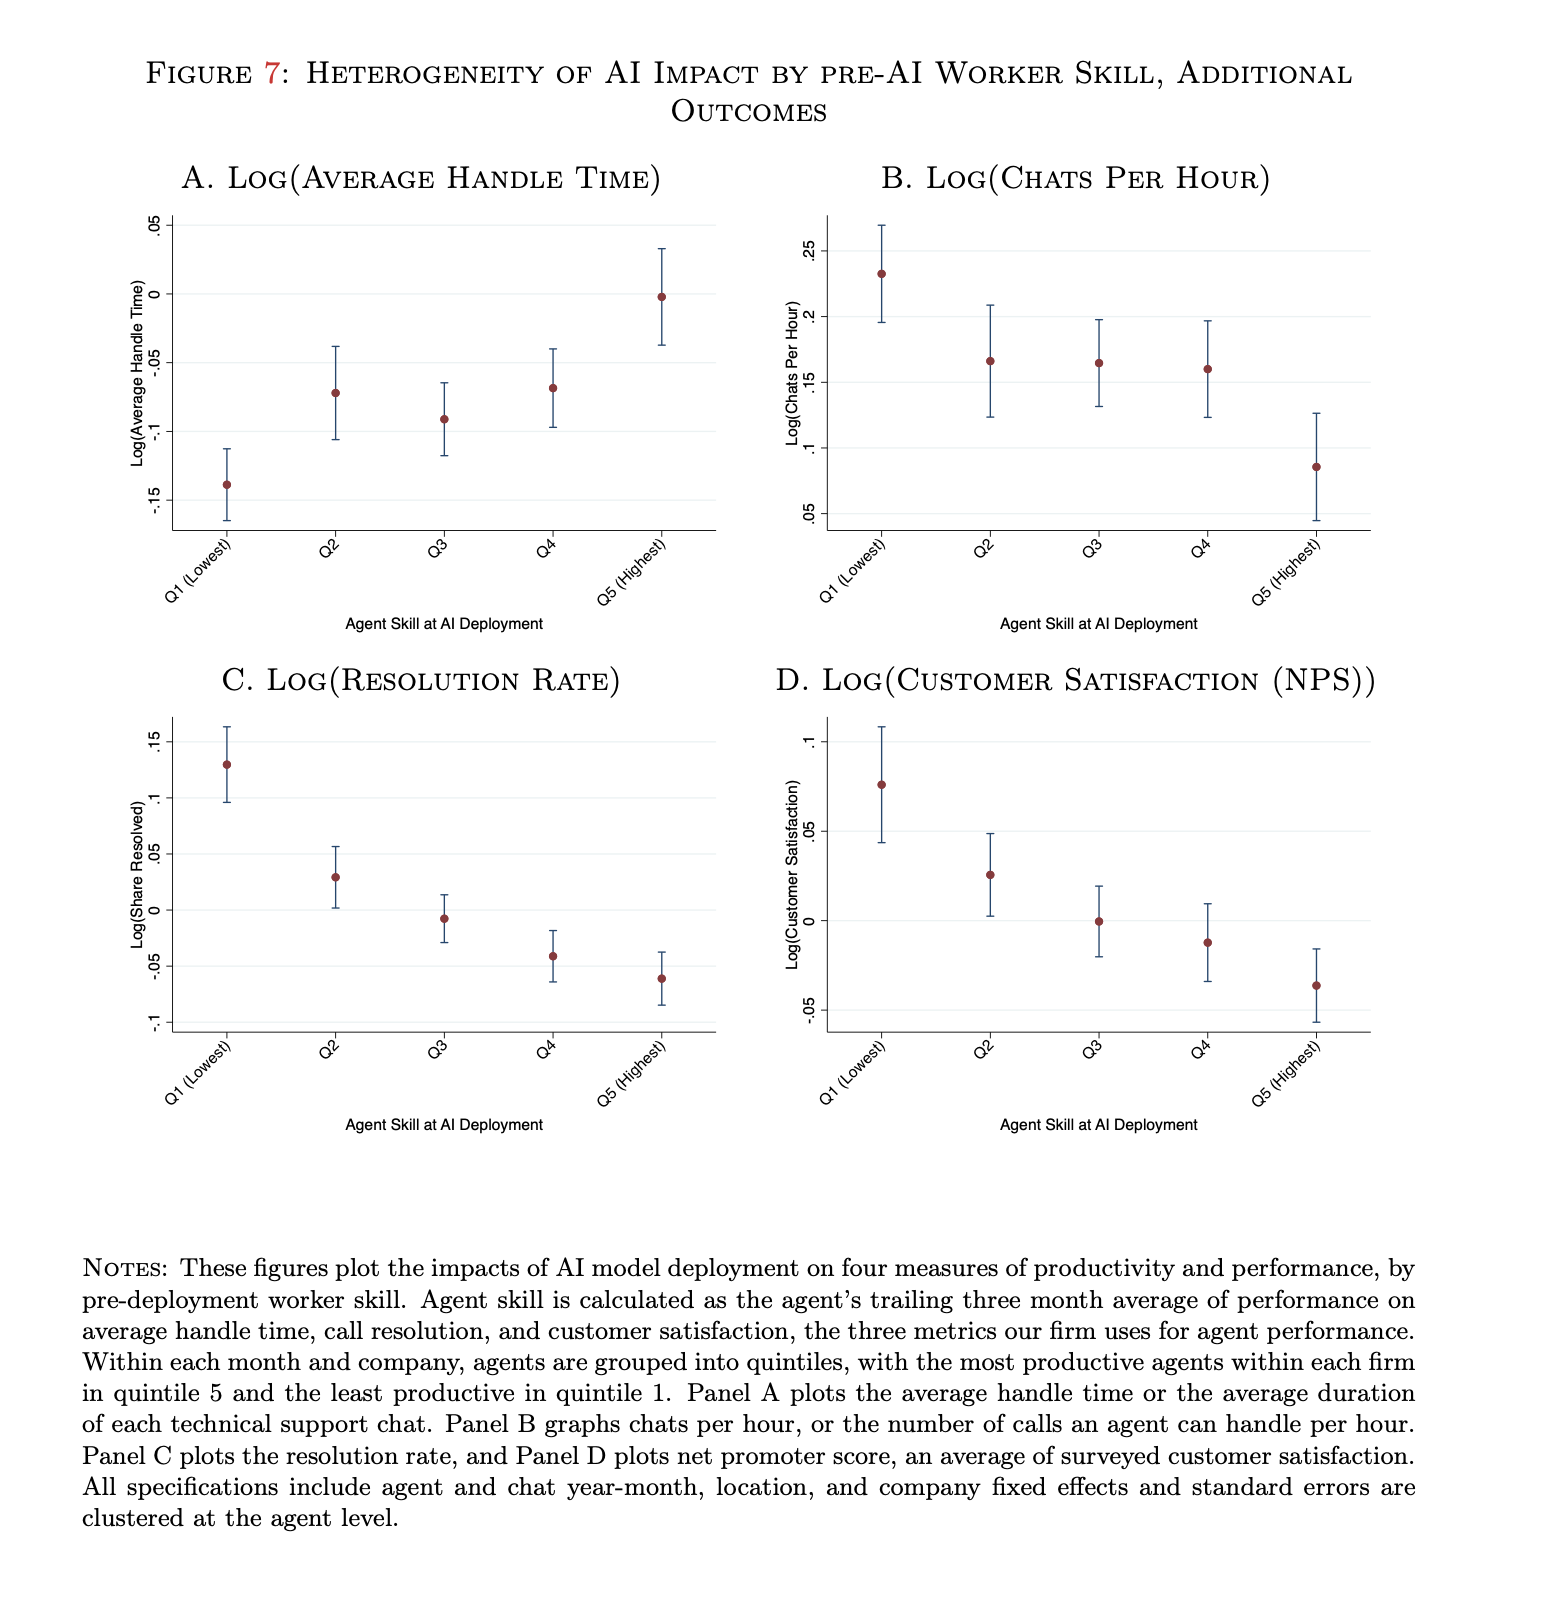
\includegraphics[scale=0.25]{./lecture_includes/brynn6}
\end{center}
\end{frame}

\begin{frame}{Heterogeneity by Worker Tenure}
\begin{center}
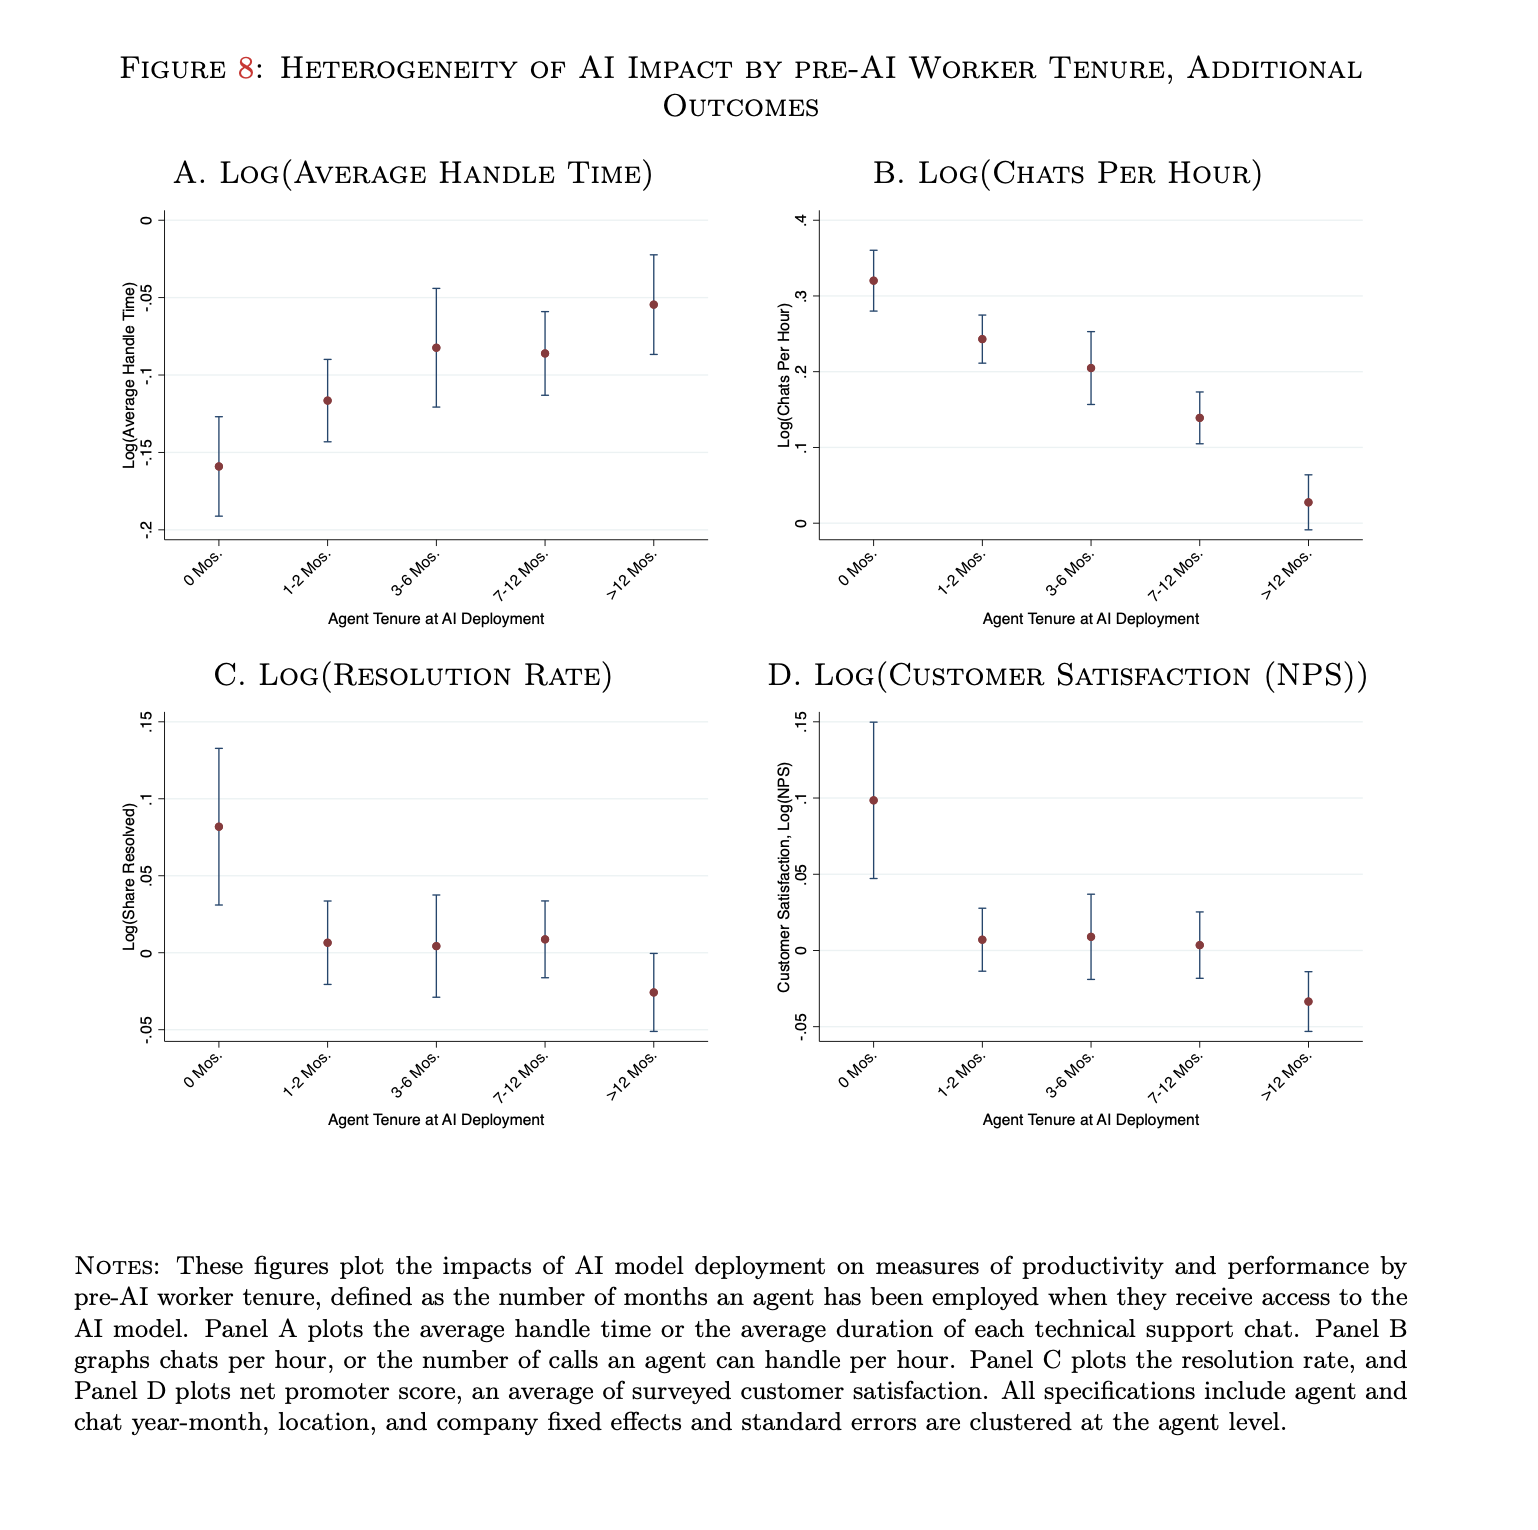
\includegraphics[scale=0.35]{./lecture_includes/brynn7}
\end{center}
\end{frame}



\begin{frame}{Sentiment}
\begin{center}
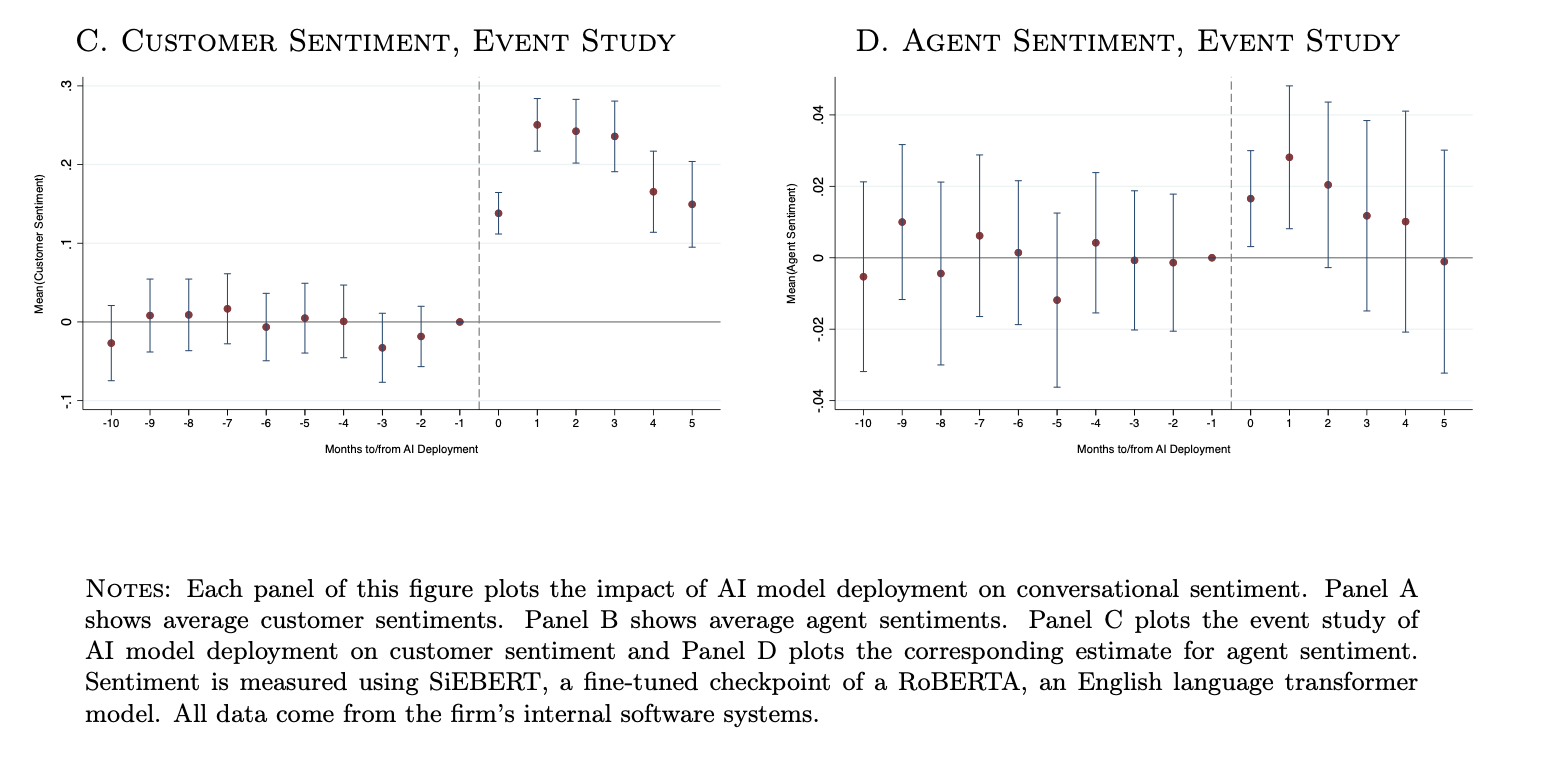
\includegraphics[scale=0.35]{./lecture_includes/brynn8}
\end{center}
\end{frame}


\begin{frame}{Sentiment}
\begin{center}
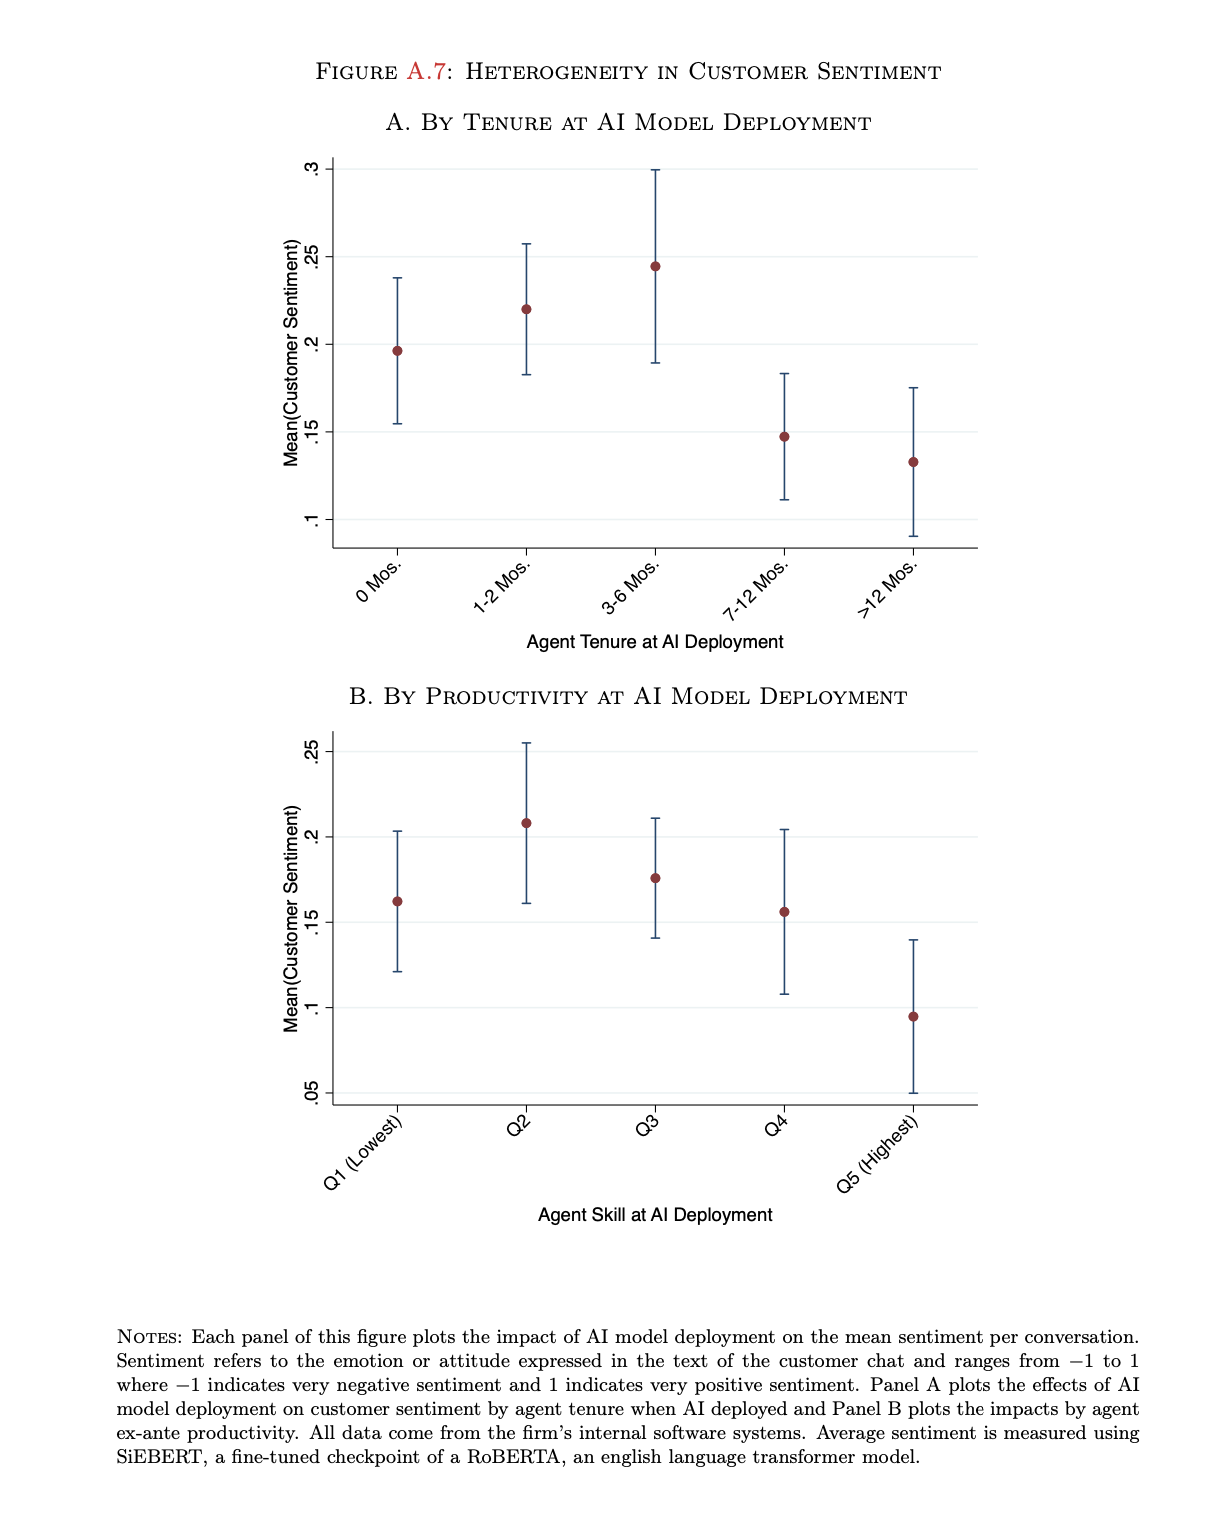
\includegraphics[scale=0.3]{./lecture_includes/brynn11}
\end{center}
\end{frame}


\begin{frame}{Manager Assistance}
\begin{center}
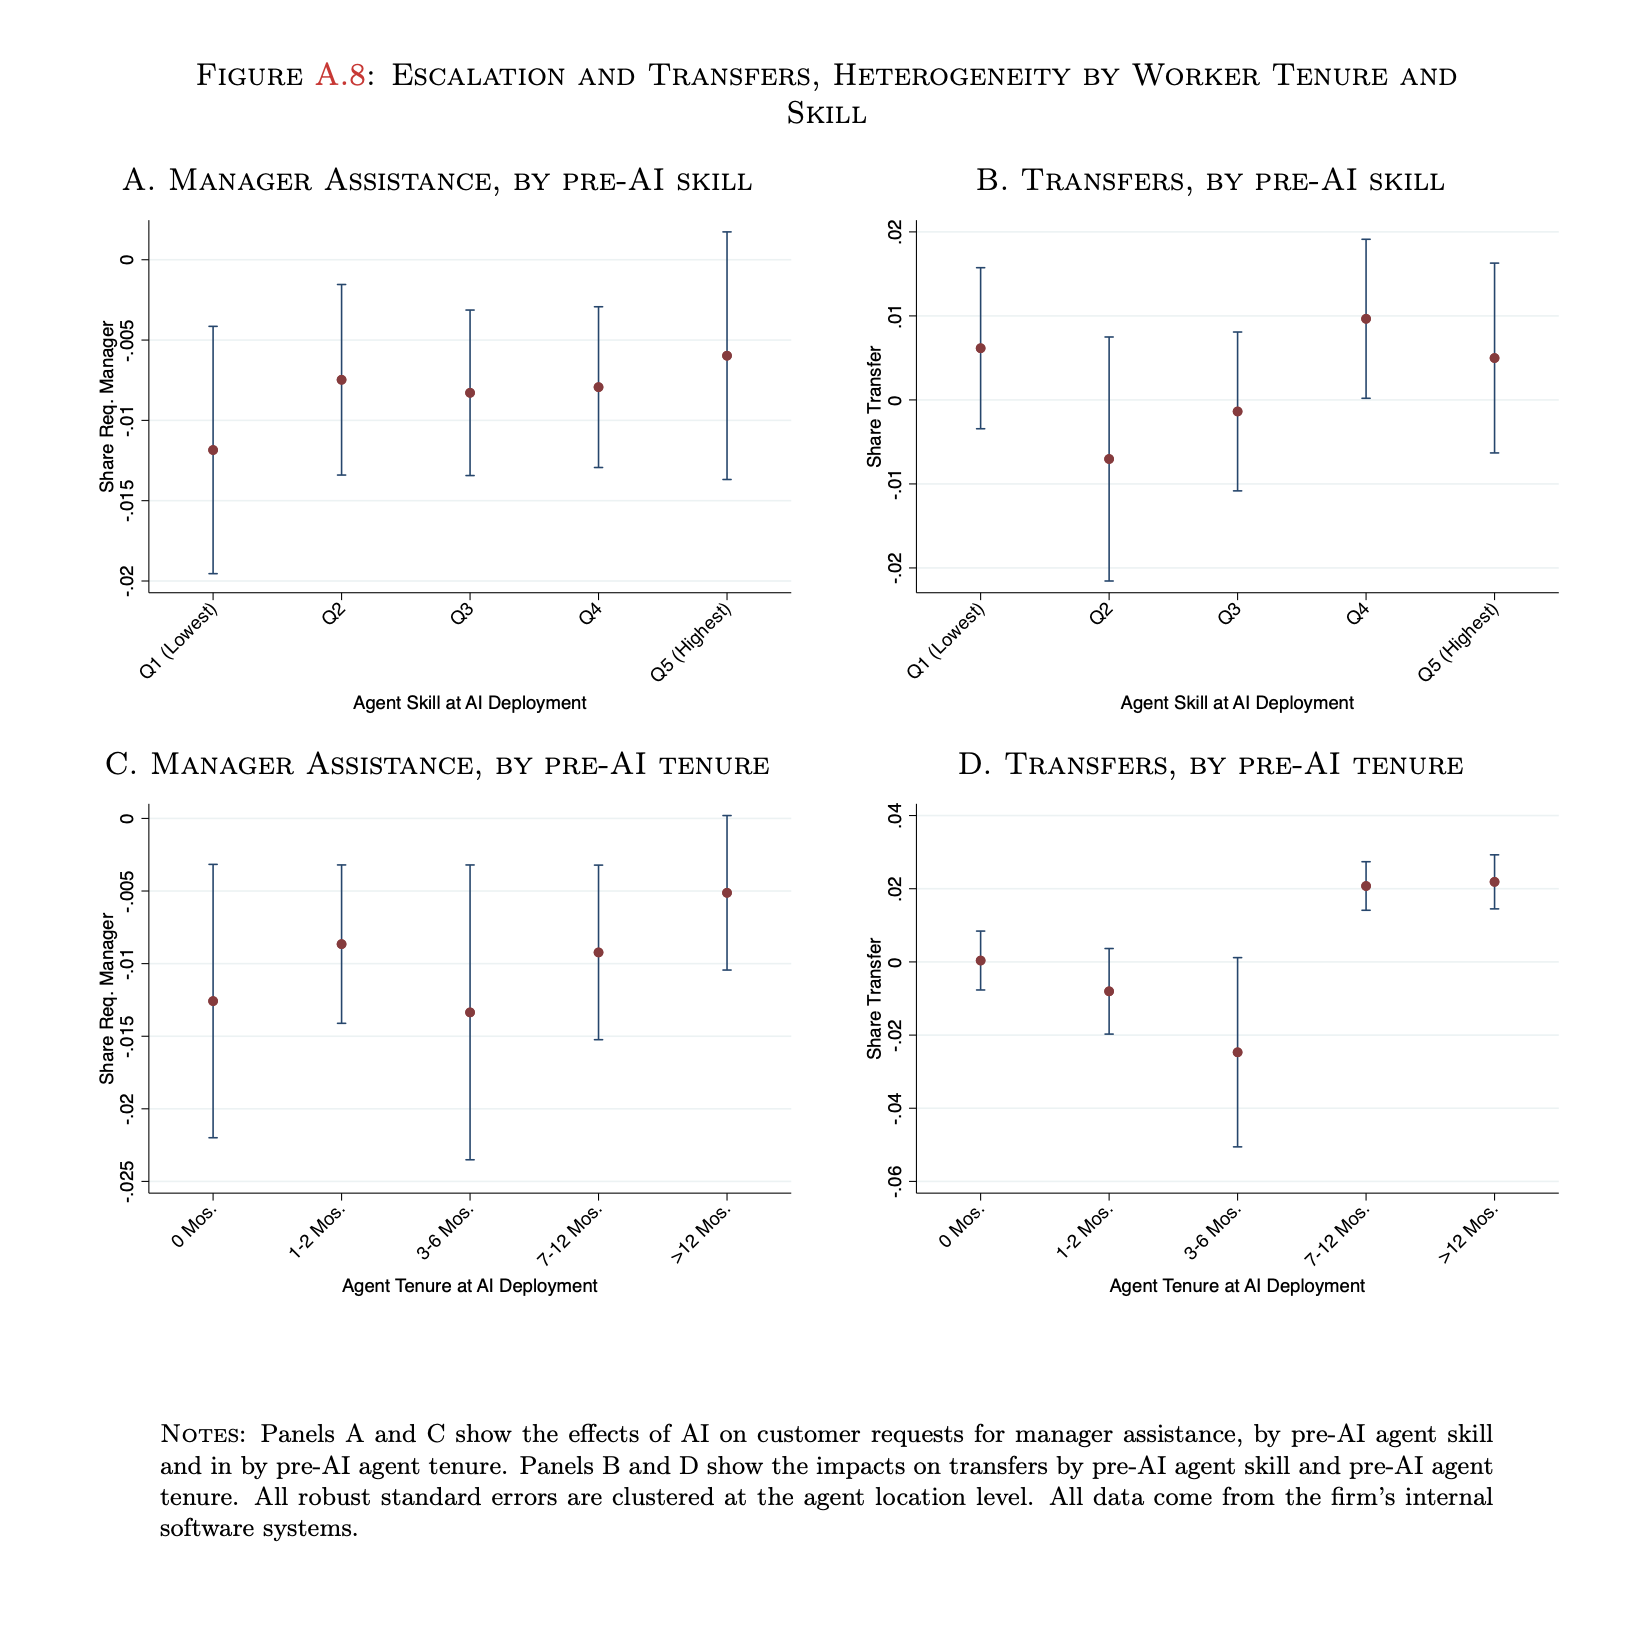
\includegraphics[scale=0.25]{./lecture_includes/brynn9}
\end{center}
\end{frame}


\begin{frame}{Outcomes}

\begin{itemize}

\item Across many dimensions, worker productivity rose
\item And the productivity increases were higher for the least skilled workers -- just like we had seen in the experiment
\item They suggest that generative AI ``reallocated experience'' to the least experienced workers making them essentially appear as though they had been their awhile
\item Findings suggest that it improves customer sentiment, reduces requests for managerial intervention, and improves employee retention
\item Still unclear how generalizeable this is, and what impact we should see on overall aggregate employment as this was AI assisted, not AI alone

\end{itemize}

\end{frame}



\begin{frame}{Facebook vs AI Event Study}
\begin{multicols}{2}

\begin{figure}
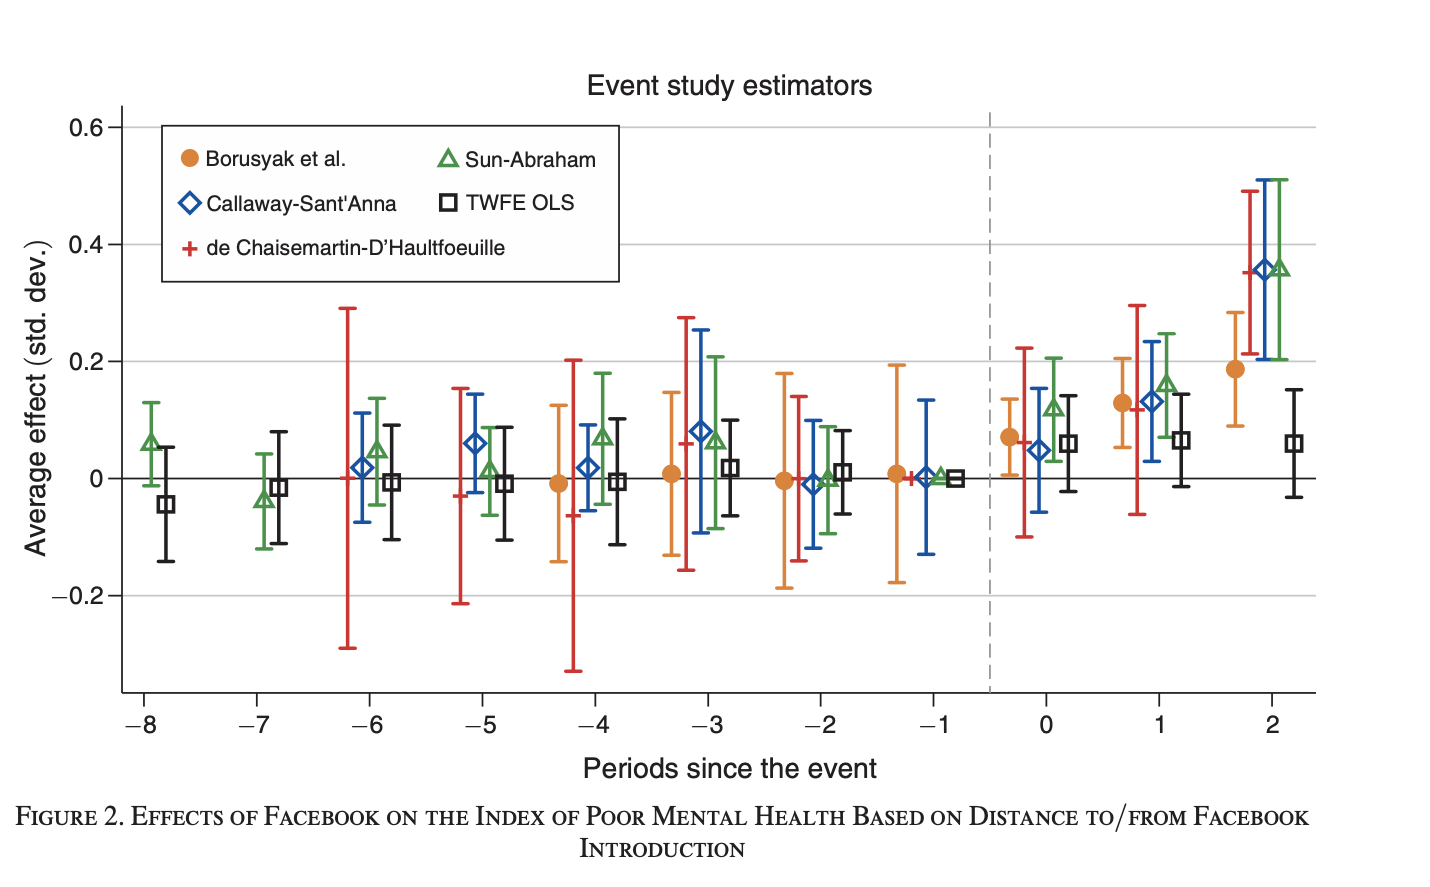
\includegraphics[width=0.95\linewidth, keepaspectratio]{./lecture_includes/facebook_3}
\end{figure}

\begin{figure}
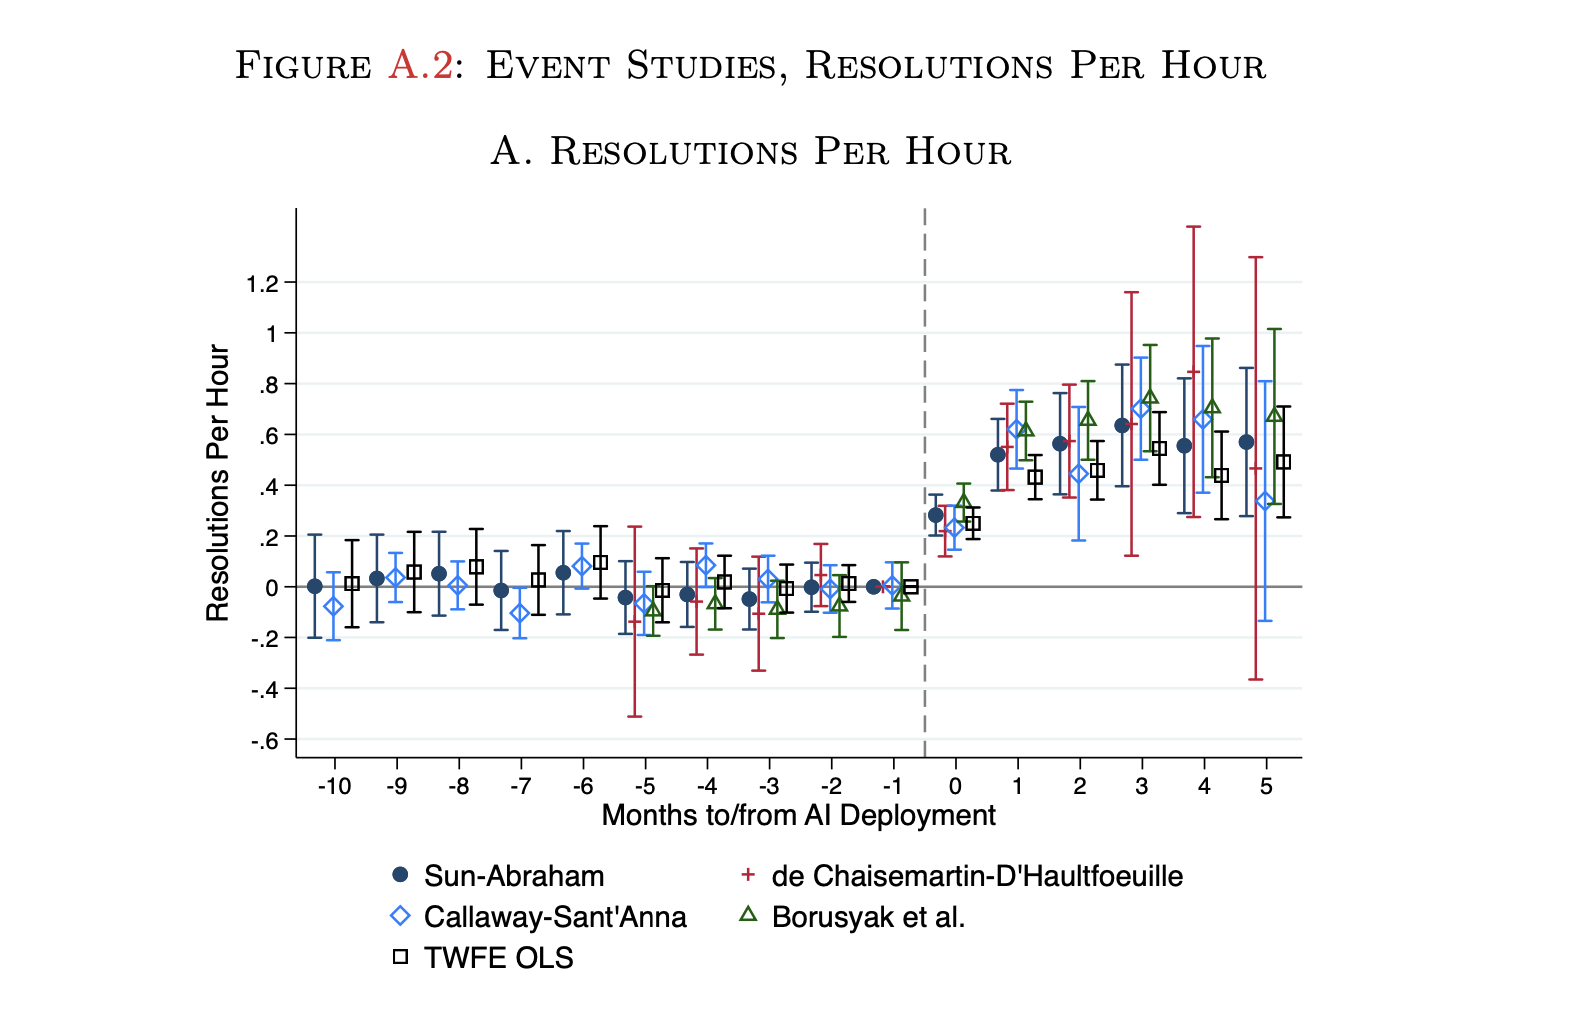
\includegraphics[width=0.95\linewidth, keepaspectratio]{./lecture_includes/genai_alldid}
\end{figure}

\end{multicols}

\begin{itemize}
\item Facebook TWFE estimate is biased downward; AI TWFE is unbiased
\item Recall what TWFE needs:
	\begin{enumerate}
	\item SUTVA (no interference)
	\item No Anticipation (baseline is untreated)
	\item Parallel Trends
	\item \textcolor{red}{Homogeneous Treatment Profiles}: All cohorts have the same dynamic treatment effects
	\end{enumerate}
\end{itemize}

\end{frame}

\begin{frame}{Sun and Abraham decomposition}

\begin{eqnarray*}
\mu_g &=& \underbrace{\sum_{l \in g} \sum_{e} w^g_{e,l} \big ( E[Y_{i,e+l} - Y^{\infty}_{i,0} | E_i = e] - E[Y^{\infty}_{i,e+l} - Y^{\infty}_{i,0}] \big )}_{\mathclap{\text{Targets}}} \\
&+& \underbrace{\sum_{g' \neq g} \sum_{l \in g'} \sum_e w^g_{e,l} \big ( E[Y_{i,e+l} - Y^{\infty}_{i,0} | E_i=e] - E[Y^{\infty}_{i,e+l} - Y^{\infty}_{i,0}] \big )}_{\mathclap{\text{Contamination from other leads and lags}}} \\
&+&  \underbrace{\sum_{l \in g^{excl}} \sum_{e} w^g_{e,l} \big ( E[Y_{i,e+l} - Y^{\infty}_{i,0} | E_i=e] - E[Y^{\infty}_{i,e+l} - Y^{\infty}_{i,0}] \big )}_{\mathclap{\text{Contamination from dropped periods}}} 
\end{eqnarray*}

Any relative time indicator (e.g., $g=-2$) is equal to the sum of three (weighted) types of difference-in-differences calculations
\end{frame}


\begin{frame}{Sun and Abraham decomposition}

\begin{eqnarray*}
\mu_g &=& \underbrace{\sum_{l \in g} \sum_e w^g_{e,l} CATT_{e,l}}_{\mathclap{\text{Desirable}}} \\
&& + \underbrace{\sum_{g' \neq g, g' \in G} \sum_{l' \in g'} \sum_e w^g_{e,l'}  CATT_{e,l'}}_{\mathclap{\text{Bias from other specified bins}}} \\
&&+ \underbrace{\sum_{l' \in g^{excl}} \sum_e w^g_{e,l'} CATT_{e,l'}}_{\mathclap{\text{Bias from dropped relative time indicators}}}
\end{eqnarray*}

Parallel trends turns each diff-in-diff into a cohort specific ATT (i.e., CATT)

\end{frame}

\begin{frame}{Sun and Abraham decomposition}

\begin{eqnarray*}
\mu_g &=& \underbrace{\sum_{l \in g} \sum_e w^g_{e,l} CATT_{e,l}}_{\mathclap{\text{Desirable}}} \\
&& + \underbrace{\sum_{g' \neq g, g' \in G} \sum_{l' \in g'} \sum_e w^g_{e,l'}  CATT_{e,l'}}_{\mathclap{\text{Bias from other specified bins}}} \\
&&+ \underbrace{\sum_{l' \in g^{excl}} \sum_e w^g_{e,l'} CATT_{e,l'}}_{\mathclap{\text{Bias from dropped relative time indicators}}}
\end{eqnarray*}

No Anticipation causes third row to be zero; causes all $g<0$ to be zero too

\end{frame}

\begin{frame}{Sun and Abraham decomposition}

\begin{eqnarray*}
\mu_g &=& \sum_{l \in g} w^g_l ATT_l \\
&&+ \sum_{g' \neq g} \sum_{l' \in g'} w^g_{l'} ATT_{l'} \\
&&+ \sum_{l' \in g^{excl}} w^g_{l'}ATT_{l'}
\end{eqnarray*}

Treatment effect homogeneity profiles cause all $CATT_{e,l}$ to be the same; therefore $ATT_{l}$ and not dependent on the timing

\end{frame}

\begin{frame}{What will cause second row to vanish?}

\begin{eqnarray*}
\mu_g &=& \sum_{l \in g} w^g_l ATT_l \\
&&+ \sum_{g' \neq g} \sum_{l' \in g'} w^g_{l'} ATT_{l'} \\
&&+ \sum_{l' \in g^{excl}} w^g_{l'}ATT_{l'}
\end{eqnarray*}

Second row weights sum to 0 (for each $l$ bin) meaning some are negative. But if they're all the same for each $l$ bin, then they cancel out. So question is why would they ever be the same?

\end{frame}

\begin{frame}{Two ways TWFE becomes unbiased}

\begin{enumerate}
\item Not a lot of heterogeneity.  Maybe in your application there isn't a lot of treatment effect heterogeneity and so trivially there are no unique $CATT_{e,l}$ 
\item \textbf{Randomization of the treatment}. If the treatment rolled out to different groups \emph{randomly}, then it implies:
	\begin{eqnarray*}
	E[Y^0|D=1] &=&E[Y^0|D=0] = E[Y^0] \\
	E[Y^1|D=1] &=&E[Y^1|D=0] = E[Y^1] \\
	E[\delta | D=1] &=&E[\delta | D=0] = E[\delta]
	\end{eqnarray*}
\item Mean covariates and potential outcomes are distributed equally for all groups under randomization, in other words, which causes treatment effect homogeneity profile, and therefore TWFE is unbiased
\item Diff-in-diff does not require this -- it's more than we need -- but if the rollout was random, then there are good reasons to use TWFE as it's more efficient since it uses more variation in the data

\end{enumerate}

\end{frame}

\begin{frame}{Facebook vs Generative AI Rollout}

\begin{itemize}
\item We know from the paper that early adopters of Facebook had \emph{worse} baseline mental health; this could mean that the treatment effect profiles will be different from later adopters, hence why TWFE was biased
\item But is the firm targeting the best or worst customer service agents and giving them chatbots earlier than later?
\item That's the question -- is the selection into treatment based on the dynamic profiles? Then TWFE is likely biased, but that is not guaranteed to be the case
\item And homogenous treatment effects also, regardless of the profiles, also addresses this


\end{itemize}

\end{frame}


\begin{frame}{So why not then TWFE?}

\begin{itemize}
\item Why not just assume randomized roll outs? 
\item You don't assume randomization -- it either was a literal, physical randomized roll out or it was not
\item And assuming homogenous treatment profiles is to make a strong statement about some underlying production functions \emph{about which we know very little beforehand}
\item Assuming constant treatment effects is a strong assumption and unnecessary
\end{itemize}

\end{frame}
	



\section{Concluding remarks}



\begin{frame}{DiD vs ATT}

\begin{itemize}

\item We learned that difference-in-differences was just four averages and three subtractions
\item But it was also a specific regression specification
\item We saw that difference-in-differences could be used to estimate average treatment effects 
\item But the DiD equation is distinct from the ATT parameter we care about

\end{itemize}

\end{frame}


\begin{frame}{Parallel Trends}

\begin{itemize}

\item DiD only was equal to the ATT if the parallel trends assumption was true
\item But it's not verifiable so it's a difficult assumption
\item Parallel trends is not something a statistical model fixes -- it's something a control group fixes
\item Some comparison groups will satisfy parallel trends, but some won't
\item Neither of the following test the actual parallel trends assumption, but ultimately you have to take a stand on the trend and these are tests that you were justified


\end{itemize}

\end{frame}

\begin{frame}{Evidence for parallel trends}



\begin{enumerate}

\item Event study graphics are placebos on the \emph{pre-treatment period}
	\begin{itemize}
	\item Plot coefficients and 95\% confidence intervals 
	\item Check if pre-trends are zero 
	\item Consider bounding if you think that's not likely (``honest diff-in-diff'' by Rambachan and Roth 2024)
	\end{itemize}
\item Falsifications are placebos on the \emph{post-treatment period}
	\begin{itemize}
	\item Assume some confounder and find a nearly identical group that should be affected by that confounder (but not eligible for the treatment)
	\item Run your diff-in-diff on that ``nearly identical'' group 
	\item Recall Miller, Johnson and Wherry using the 65 and older group as a falsification -- shouldn't they be affected by the confounder?
	\end{itemize}



\end{enumerate}

\end{frame}

\begin{frame}{Five Types of Evidence}

\begin{enumerate}
\item Show bite -- first order effects
\item Main results -- What's your study about?
\item Event study graphs -- This will be your main results and your evidence of parallel trends keeping in mind pre-trends and parallel trends are technically distinct
\item Falsifications -- If you can find falsifications, use them
\item Mechanisms -- can you find any explanation?  
\end{enumerate}

\end{frame}

\begin{frame}{Imputation methods}

\begin{itemize}

\item But what if parallel trends really isn't realistic -- what then? At minimum, then diff-in-diff is not a solution
\item We will review that next tomorrow when Kyle discusses imputation methods, including his own work
\item Thank you!
\end{itemize}

\end{frame}













\end{document}
